\documentclass[11pt]{amsart}
\usepackage[T1]{fontenc}
\usepackage{lmodern}
\usepackage{amsmath,amssymb,amsthm,mathtools}
\usepackage{microtype}
\usepackage[margin=1in]{geometry}
\usepackage{booktabs}
\usepackage{array}
\usepackage{enumitem}
\usepackage[dvipsnames]{xcolor}
\usepackage{tikz}
\usetikzlibrary{arrows.meta,calc,decorations.pathreplacing,positioning,shapes.geometric,backgrounds,fit}
\usepackage{pgfplots}
\pgfplotsset{compat=1.18}
\usepgfplotslibrary{fillbetween}
\usepackage[colorlinks=true,linkcolor=MidnightBlue,citecolor=MidnightBlue,urlcolor=MidnightBlue]{hyperref}
\usepackage[nameinlink,noabbrev]{cleveref}

\numberwithin{equation}{section}
\newtheorem{theorem}{Theorem}[section]
\newtheorem{proposition}[theorem]{Proposition}
\newtheorem{lemma}[theorem]{Lemma}
\newtheorem{corollary}[theorem]{Corollary}
\theoremstyle{definition}
\newtheorem{definition}[theorem]{Definition}
\theoremstyle{remark}
\newtheorem{remark}[theorem]{Remark}
\crefname{theorem}{Theorem}{Theorems}
\crefname{lemma}{Lemma}{Lemmas}
\crefname{proposition}{Proposition}{Propositions}
\crefname{corollary}{Corollary}{Corollaries}
\crefname{remark}{Remark}{Remarks}
\crefname{definition}{Definition}{Definitions}
\crefname{section}{Section}{Sections}
\crefname{appendix}{Appendix}{Appendices}
\crefname{figure}{Figure}{Figures}
\crefname{table}{Table}{Tables}
\crefname{step}{Step}{Steps}

% ---------------------------------------------------------------------------
% Notation
\newcommand{\R}{\mathbb R}
\newcommand{\N}{\mathbb N}
\newcommand{\ip}[2]{\langle #1,#2\rangle}
\newcommand{\norm}[1]{\lVert #1\rVert}
\newcommand{\opnorm}[1]{\lVert #1\rVert_{\mathrm{op}}}
\newcommand{\T}{\mathsf T}          % transpose
\newcommand{\one}{\mathbf 1}
\newcommand{\Tmax}{T_{\max}}
\DeclareMathOperator{\diam}{diam}
\DeclareMathOperator{\diag}{diag}
\newcommand{\res}[1]{[#1]_p}
\newcommand{\TripodoCommit}{\texttt{1e73a12}}

% Labelled hypotheses (C1)--(C5)
\newcommand{\cond}[1]{\textup{(C#1)}}

% Figure colours (colour-blind safe)
\definecolor{cblue}{HTML}{0072B2}
\definecolor{corange}{HTML}{E69F00}
\definecolor{cverm}{HTML}{D55E00}
\definecolor{cgreen}{HTML}{009E73}
\definecolor{cpurple}{HTML}{CC79A7}
\definecolor{csky}{HTML}{56B4E9}
\definecolor{cgray}{HTML}{6E6E6E}
\definecolor{clight}{HTML}{F2F2F2}

\emergencystretch=1.5em
\setlength{\abovecaptionskip}{6pt}
\hypersetup{pdfauthor={John Tripodo},
  pdftitle={Orthogonal circles and a fixed-dimensional separated-distance counterexample},
  pdfsubject={A finite fixed-dimensional counterexample to Erd\H{o}s Problem 670}}

\title[Orthogonal circles and separated distances]{Orthogonal circles and a fixed-dimensional\newline separated-distance counterexample}
\author{John Tripodo}
\date{14 October 2026}

\begin{document}

\begin{abstract}
A finite set of points in Euclidean space is \emph{distance-separated} if
the lengths of any two different unordered edges differ by at least one. Counting the
distances shows that an $n$-point distance-separated set has diameter at
least $\binom n2\approx n^2/2$, and Erd\H{o}s asked whether the diameter
must in fact be at least $(1-o(1))n^2$. Ho showed that the answer is no if
the dimension may grow with $n$. The first version of this paper then gave
counterexamples with diameter below $0.74n^2$ in a single fixed dimension.

We give a fixed-dimensional counterexample with sharper explicit parameters:
for every integer $n\ge36354$ there is a distance-separated $n$-point
set in $\R^{81794}$ with diameter below $(147/200)n^2=0.735n^2$.
The finite conclusion has an accompanying Lean~4 proof, including minimum
distance at least one for distinct points and the actual set diameter bound.

As in the first version, this construction replaces each vertex of a large
``macro'' simplex by a cluster of points. We use a standard Gram-deficit
completion to arrange those clusters on circles in mutually orthogonal
planes. The new arrangement makes every distance between two clusters
an exact, explicit, increasing function of two ``digits'', and it
reduces the number of coordinates from $9m-1$ to $3m-1$ for $m$ clusters. A
single quadratic-residue ruler then controls both the distances inside the
clusters and the digits between them. The proof is self-contained apart from
Bertrand's postulate.
\end{abstract}

\maketitle

% ===========================================================================
\section{Introduction}\label{sec:intro}

\subsection{Separated distances and the counting bound}

Let $X$ be a finite set of points in a Euclidean space $\R^d$. An
\emph{edge} of $X$ is an unordered pair $\{x,y\}$ of distinct points of $X$,
and its \emph{length} is $\norm{x-y}$. We call $X$
\emph{distance-separated} if the lengths of any two different edges differ
by at least one:
\begin{equation}\label{eq:separated}
 \bigl|\norm{x-y}-\norm{u-v}\bigr|\ge1
 \qquad\text{whenever }\{x,y\}\ne\{u,v\}\text{ are edges of }X.
\end{equation}
In particular, the $\binom{|X|}2$ edge lengths are pairwise distinct.

How small can the diameter of such a set be? There is a simple lower
bound. If $|X|\ge3$, every edge $\{x,y\}$ has length at least one: pick a
third point $z$; the edges $\{x,z\}$ and $\{y,z\}$ are different, so by
\eqref{eq:separated} and the triangle inequality
\[
 1\le\bigl|\norm{x-z}-\norm{y-z}\bigr|\le\norm{x-y}.
\]
Hence the sorted edge lengths $\ell_1<\ell_2<\cdots<\ell_N$, where
$N=\binom{|X|}2$, satisfy $\ell_1\ge1$ and $\ell_{t+1}\ge\ell_t+1$, so
$\ell_t\ge t$ for every $t$. Taking $t=N$ gives the \emph{counting bound}
\begin{equation}\label{eq:counting}
 \diam X\ge\binom{|X|}{2}=\Bigl(\frac12-o(1)\Bigr)|X|^2.
\end{equation}

On the real line the truth is twice as large: an $n$-point
distance-separated subset of $\R$ has diameter at least $n^2-3n^{3/2}$
(\cref{prop:line} below). Erd\H{o}s asked whether the same holds in every
dimension, that is, whether $\diam X\ge(1-o(1))n^2$ for every
distance-separated $n$-point set $X$ in any Euclidean space; see
Erd\H{o}s~\cite[Problem~20]{Erdos}. This is Erd\H{o}s Problem~670.

Ho~\cite{Ho} showed that the answer is negative if the ambient dimension
may grow with~$n$: for infinitely many $n$ there are distance-separated
$n$-point sets in $\R^{n^2-n}$ of diameter $(1-1/\pi^2+o(1))n^2$. Ho also
gave the stronger proved asymptotic coefficient
$(\pi+\sqrt{\pi^2-4})/(2\pi)=0.885589\ldots$ for his high-dimensional
construction~\cite[Remark~10]{Ho}. He
pointed out that this leaves the question in a \emph{fixed} dimension open
\cite[Remark~9]{Ho}. The first version of this paper~\cite{Tripodo}
constructed distance-separated $n$-point sets in $\R^{458999}$ with
diameter below $0.74n^2$ for every $n\ge68000$.

To state results in fixed dimension, define for $d\ge1$ and $n\ge3$
\[
 \Delta_d(n)=\inf\bigl\{\diam X:\ X\subset\R^d,\ |X|=n,\
                    X\text{ is distance-separated}\bigr\}.
\]
The infimum is over a nonempty class: for instance
$\{1,2,4,\dots,2^{n-1}\}\subset\R$ is distance-separated, since its
differences $2^b-2^a$ are distinct integers. Padding with zero coordinates
embeds $\R^d$ in $\R^{d+1}$, so $\Delta_d(n)$ is nonincreasing in~$d$.
The counting bound gives $\Delta_d(n)\ge\binom n2$ for every~$d$.
The fixed-dimensional question asks whether, for every fixed~$d$,
\[
 \liminf_{n\to\infty}\frac{\Delta_d(n)}{n^2}\ge1,
\]
equivalently whether $\Delta_d(n)\ge(1-o(1))n^2$ as $n\to\infty$.
That first construction disproved this in one fixed dimension; the theorem
below gives a smaller explicit dimension and coefficient for all
sufficiently large~$n$.

\subsection{Results}

The finite result is an explicit improvement in both ambient dimension and
diameter coefficient over the first version of this paper.

\begin{theorem}[A fixed-dimensional counterexample]\label{thm:explicit}
For every integer $n\ge36354$ there is a distance-separated set
$X\subset\R^{81794}$ with $|X|=n$ and
\[
 \diam X<\frac{147}{200}\,n^2=0.735\,n^2.
\]
\end{theorem}

\subsection{The idea: a two-digit counter}\label{sec:idea}

Here is the construction in outline; \cref{fig:overview,fig:counter}
illustrate it. We build a set of $n=mk$ points, arranged in $m$
\emph{clusters} of $k$ points each. The number $m$ of clusters is fixed
(it determines the dimension, $3m-1$), while the cluster size $k$ grows
with~$n$.

\emph{The macro skeleton.} Start with the $M=\binom m2$ consecutive
target lengths
\[
 S(K+1),\ S(K+2),\ \dots,\ S(K+M).
\]
Here $K$ is a large offset. The edges are numbered $1,\dots,M$ in
\emph{colexicographic} order (\cref{fig:colex}). As in the first
version~\cite{Tripodo}, a Gram estimate realizes the required macro vertices
$q_A$ in $\R^{m-1}$. Their actual distances are shortened to
$\|q_A-q_B\|=\sqrt{D_{AB}^2-2\rho^2}$, where $D_{AB}=K+\ell_{AB}$ and
$\rho=R/S$. This shortening offsets the radius $R$ of the circles and
leaves the displayed consecutive values as the cross-edge baselines.

\emph{Clusters.} Replace each macro vertex $Sq_A$ by a cluster of $k$
points $x_{A0},\dots,x_{A,k-1}$ lying on a small circle near $Sq_A$. The
set now has two kinds of edges: \emph{local} edges, inside one cluster,
whose lengths are comparatively short; and \emph{cross} edges, between
two clusters $A<B$, whose lengths are close to $SD_{AB}$, where
$D_{AB}=K+(\text{label of the macro edge }AB)$.

\emph{Cross lengths as a two-digit number.} The positions on the circles
are chosen so that, for $A<B$,
\begin{equation}\label{eq:counter-idea}
 \norm{x_{Ai}-x_{Bj}}\;\approx\;
 SD_{AB}\;+\;s^2k\,f_{Ai}\;+\;s\,f_{Bj},
\end{equation}
where $s>1$ is a number slightly larger than one and the \emph{digits}
$f_{A0}<f_{A1}<\dots<f_{A,k-1}$ are real numbers that increase in steps of
about one and span an interval of length less than $k$. Read
\eqref{eq:counter-idea} as a two-digit counter (\cref{fig:counter}).
Increasing the \emph{fine digit} $j$ by one increases the length by
about $s$, slightly more than one. Increasing the \emph{coarse digit} $i$ by one
increases it by about $s^2k$, which is more than the whole range, about
$sk$, of the fine digit. So the $k^2$ cross lengths between $A$ and $B$
are separated and fill a \emph{block} of width about $s^2k^2$ around
$SD_{AB}$. Consecutive blocks are $S$ apart, and the choice $S=s^3k^2$
leaves room between them. Finally, the local lengths lie far below all
cross lengths and are separated by a separate argument.

\emph{The diameter coefficient.} The largest cross length is about
\[
 S(K+M)\approx s^3k^2\Bigl(K+\frac{m^2}2\Bigr)
 =s^3\Bigl(\frac12+\frac K{m^2}\Bigr)(mk)^2.
\]
For the finite theorem we take $s=9/8$, $m\ge18177$, and
$K=\lceil m(m-1)/64\rceil$. The resulting leading coefficient is
$s^3(1/2+1/64)=24057/32768<147/200$; the explicit finite margin
absorbs the lower-order terms (\cref{sec:explicit}).

\emph{The difficulty, and how orthogonal circles remove it.} Write the
points as $x_{Ai}=Sq_A+\eta_{Ai}$ with small perturbations $\eta_{Ai}$.
Then
\[
 \norm{x_{Ai}-x_{Bj}}^2
 =S^2\norm{q_A-q_B}^2
  +2S\ip{q_A-q_B}{\eta_{Ai}-\eta_{Bj}}
  +\norm{\eta_{Ai}-\eta_{Bj}}^2.
\]
The middle term is linear in the perturbations and can produce the two
digits. The last term, however, contains the interaction
$-2\ip{\eta_{Ai}}{\eta_{Bj}}$, which depends on $i$ and $j$
\emph{jointly} and spoils the digit structure. We remove it completely:
we put all the points of cluster $A$ on a circle of a common radius $R$,
in a plane orthogonal to the planes of all other clusters. Then
$\norm{\eta_{Ai}-\eta_{Bj}}^2=2R^2$ is a constant, which we absorb by
slightly shortening the macro distances. \Cref{lem:completion} shows that
these mutually orthogonal circles cost only $2m$ extra coordinates, while
allowing the prescribed macro-space tilts when their complete direction
matrix has operator norm at most $R$, which is what creates the digits.
The result is the
\emph{exact} formula (\cref{sec:criterion})
\begin{equation}\label{eq:exact-idea}
 \norm{x_{Ai}-x_{Bj}}=\sqrt{\nu^2+2\nu T},
 \qquad \nu=SD_{AB},\quad T=s^2kf_{Ai}+sf_{Bj}.
\end{equation}
This is not linear in $T$, and its deviation from $\nu+T$ is not bounded
as $k\to\infty$. But it is a fixed increasing function of $T$, with
derivative close to one, and that is all the counter needs
(\cref{rem:error}).

Finally, the local lengths are chords of the circles, determined by
differences of the angles. We choose the angles from a quadratic-residue
ruler in the spirit of Erd\H{o}s and Tur\'an~\cite{ErdosTuran}, all of whose
differences are distinct integers. The same ruler, read through a sine,
also supplies the digits $f_{Ai}$. So one ruler serves both purposes.

\begin{figure}[t]
\centering
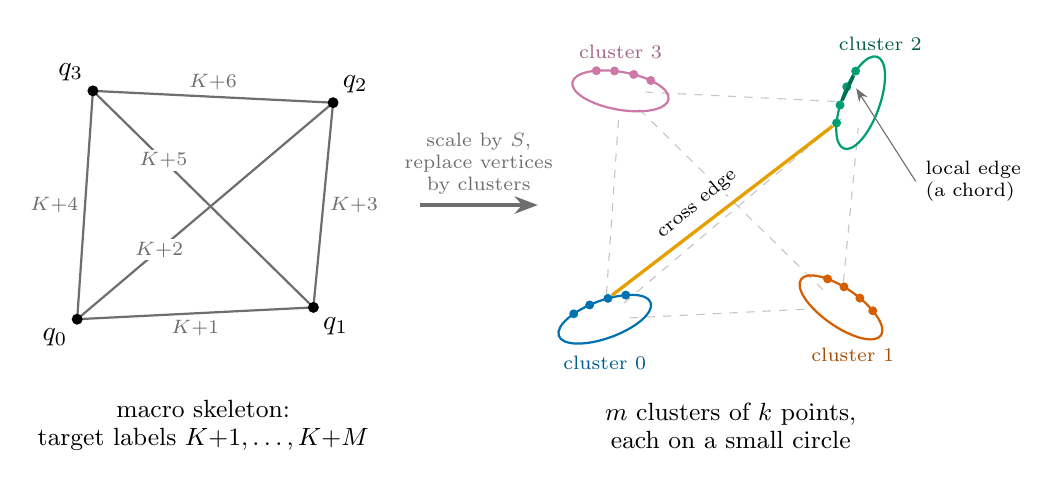
\begin{tikzpicture}[
  vtx/.style={circle,fill=black,inner sep=1.4pt},
  lab/.style={font=\scriptsize,fill=white,inner sep=1pt},
  >=Stealth]
 % ---------- left: macro skeleton ----------
 \begin{scope}
  \coordinate (q0) at (0,0);
  \coordinate (q1) at (3.0,0.15);
  \coordinate (q2) at (3.25,2.75);
  \coordinate (q3) at (0.2,2.9);
  \draw[cgray,thick] (q0)--(q1) node[lab,midway,below=1pt] {$K{+}1$};
  \draw[cgray,thick] (q0)--(q2) node[lab,pos=0.32] {$K{+}2$};
  \draw[cgray,thick] (q1)--(q2) node[lab,midway,right=1pt] {$K{+}3$};
  \draw[cgray,thick] (q0)--(q3) node[lab,midway,left=1pt] {$K{+}4$};
  \draw[cgray,thick] (q1)--(q3) node[lab,pos=0.68] {$K{+}5$};
  \draw[cgray,thick] (q2)--(q3) node[lab,midway,above=1pt] {$K{+}6$};
  \foreach \i in {0,...,3} \node[vtx] at (q\i) {};
  \node[below left=0pt] at (q0) {$q_0$};
  \node[below right=0pt] at (q1) {$q_1$};
  \node[above right=0pt] at (q2) {$q_2$};
  \node[above left=0pt] at (q3) {$q_3$};
  \node[font=\small,align=center] at (1.6,-1.35) {macro skeleton:\\[-1pt] target labels $K{+}1,\dots,K{+}M$};
 \end{scope}
 % ---------- arrow ----------
 \draw[->,very thick,cgray] (4.35,1.45) -- node[above,font=\scriptsize,align=center]{scale by $S$,\\ replace vertices\\ by clusters} (5.85,1.45);
 % ---------- right: clusters ----------
 \begin{scope}[xshift=6.7cm]
  \coordinate (c0) at (0,0);
  \coordinate (c1) at (3.0,0.15);
  \coordinate (c2) at (3.25,2.75);
  \coordinate (c3) at (0.2,2.9);
  \foreach \u/\w in {0/1,0/2,1/2,0/3,1/3,2/3}
     \draw[cgray!40,thin,dashed,shorten >=0.32cm,shorten <=0.32cm] (c\u)--(c\w);
  \foreach \i/\rot/\col in {0/20/cblue,1/-35/cverm,2/70/cgreen,3/-10/cpurple}{
    \begin{scope}[shift={(c\i)},rotate=\rot]
      \draw[\col,thick] (0,0) ellipse (0.62 and 0.24);
      \foreach \ang [count=\jj from 0] in {55,78,101,124}
        \node[circle,fill=\col,inner sep=1.15pt] (p\i\jj) at ({0.62*cos(\ang)},{0.24*sin(\ang)}) {};
    \end{scope}
  }
  \draw[corange,very thick] (p01) -- (p23);
  \node[font=\scriptsize,fill=white,inner sep=1pt,rotate=40] at ($(p01)!0.45!(p23)+(-0.18,0.2)$) {cross edge};
  \draw[cgreen!70!black,very thick] (p20) -- (p22);
  \node[font=\scriptsize,align=left,anchor=west] (le) at (3.95,1.75) {local edge\\(a chord)};
  \draw[cgray,->,thin] (le.west) -- ($(p21)+(0.12,-0.02)$);
  \node[font=\scriptsize,text=cblue!80!black] at ($(c0)+(0,-0.55)$) {cluster $0$};
  \node[font=\scriptsize,text=cverm!80!black] at ($(c1)+(0.15,-0.6)$) {cluster $1$};
  \node[font=\scriptsize,text=cgreen!60!black] at ($(c2)+(0.25,0.75)$) {cluster $2$};
  \node[font=\scriptsize,text=cpurple!80!black] at ($(c3)+(0,0.5)$) {cluster $3$};
  \node[font=\small,align=center] at (1.6,-1.35) {$m$ clusters of $k$ points,\\[-1pt] each on a small circle};
 \end{scope}
\end{tikzpicture}
\caption{A schematic picture with $m=4$ clusters of $k=4$ points; it is
not to scale. Left: the labels $D_{AB}=K+1,\dots,K+\binom m2$ occur in
colexicographic order (\cref{fig:colex}). The actual macro distances are
$\sqrt{D_{AB}^2-2(R/S)^2}$, before scaling by $S$. Right: each scaled
macro vertex is replaced by $k$ points on a circle of radius $R$.
The circles lie in mutually orthogonal planes, which is not visible in
this planar drawing. The radius is small compared with the macro-edge
lengths $SK$, although $R/S$ is large for the chosen parameters.}
\label{fig:overview}
\end{figure}

\begin{figure}[t]
\centering
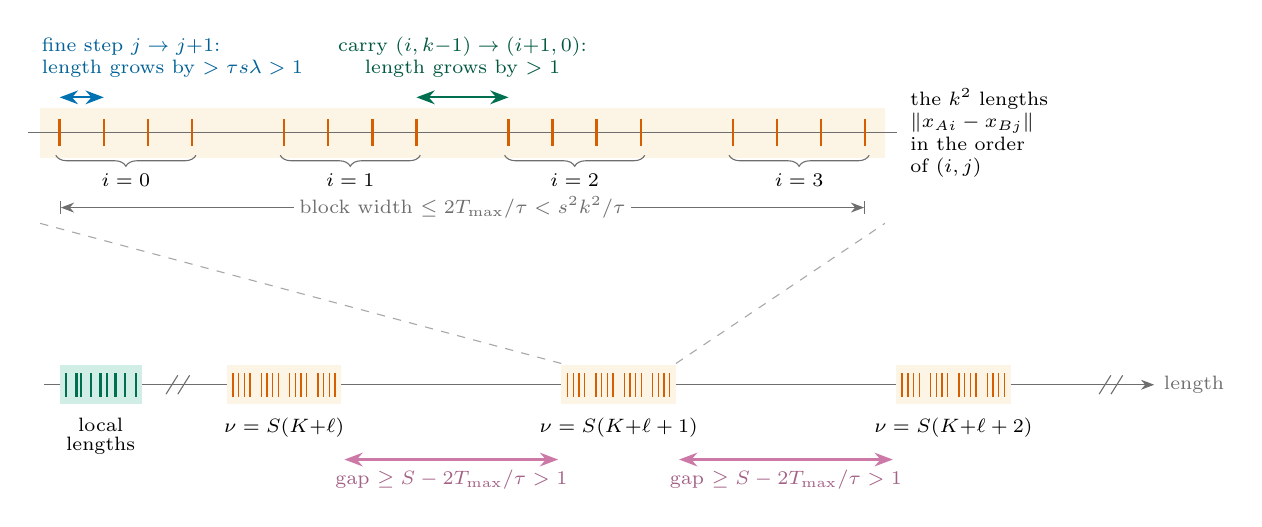
\begin{tikzpicture}[>=Stealth,
   tick/.style={line width=0.9pt},
   brace/.style={decorate,decoration={brace,amplitude=4pt,raise=1pt}}]
 % ===== zoomed block (top) =====
 \def\zc{2.85}\def\zf{0.56}% coarse and fine steps (zoom)
 \begin{scope}[yshift=3.2cm]
   \fill[corange!10] (-0.25,-0.32) rectangle ({3*\zc+3*\zf+0.25},0.32);
   \draw[cgray] (-0.4,0) -- ({3*\zc+3*\zf+0.4},0);
   \foreach \i in {0,...,3}{
     \foreach \j in {0,...,3}{
        \draw[tick,cverm] ({\i*\zc+\j*\zf},-0.17) -- ++(0,0.34);
     }
     \draw[brace,cgray] ({\i*\zc+3*\zf+0.05},-0.25) -- ({\i*\zc-0.05},-0.25)
        node[midway,below=4pt,font=\scriptsize,text=black] {$i=\i$};
   }
   % fine step annotation (between j=0 and j=1 of i=0)
   \draw[<->,cblue,thick] (0,0.45) -- (\zf,0.45);
   \node[font=\scriptsize,text=cblue!85!black,anchor=south west,align=left] at (-0.35,0.58)
       {fine step $j\to j{+}1$:\\ length grows by $>\tau s\lambda>1$};
   % carry annotation (between i=1 and i=2)
   \draw[<->,cgreen!70!black,thick] ({\zc+3*\zf},0.45) -- ({2*\zc},0.45);
   \node[font=\scriptsize,text=cgreen!55!black,anchor=south,align=center] at ({1.5*\zc+1.5*\zf},0.58)
       {carry $(i,k{-}1)\to(i{+}1,0)$:\\ length grows by $>1$};
   % block width
   \draw[|<->|,cgray] (0,-0.95) -- ({3*\zc+3*\zf},-0.95)
     node[midway,fill=white,font=\scriptsize,inner sep=2pt] {block width $\le 2\Tmax/\tau<s^2k^2/\tau$};
   \node[font=\scriptsize,anchor=west,align=left] at ({3*\zc+3*\zf+0.45},0)
       {the $k^2$ lengths\\ $\norm{x_{Ai}-x_{Bj}}$\\ in the order\\ of $(i,j)$};
 \end{scope}
 % ===== overview line (bottom) =====
 \def\sc{0.36}\def\sf{0.072}\def\Sgap{4.25}\def\bz{2.2}
 % zoom lines
 \draw[cgray!60,dashed] (\bz+\Sgap-0.08,0.27) -- (-0.25,2.05);
 \draw[cgray!60,dashed] ({\bz+\Sgap+3*\sc+3*\sf+0.08},0.27) -- ({3*\zc+3*\zf+0.25},2.05);
 \draw[cgray,->] (-0.2,0) -- (13.9,0) node[right,font=\scriptsize] {length};
 % local lengths
 \fill[cgreen!18] (0,-0.25) rectangle (1.05,0.25);
 \foreach \x in {0.08,0.21,0.27,0.4,0.52,0.6,0.71,0.83,0.97} \draw[tick,cgreen!70!black] (\x,-0.15)--++(0,0.3);
 \node[font=\scriptsize,align=center,below] at (0.52,-0.3) {local\\[-1pt] lengths};
 \draw[cgray] (1.35,-0.12)--(1.5,0.12) (1.5,-0.12)--(1.65,0.12);
 % blocks
 \foreach \b/\lab in {0/{\ell},1/{\ell+1},2/{\ell+2}}{
   \pgfmathsetmacro{\xs}{\bz+\b*\Sgap}
   \fill[corange!10] (\xs-0.08,-0.25) rectangle ({\xs+3*\sc+3*\sf+0.08},0.25);
   \foreach \i in {0,...,3}{\foreach \j in {0,...,3}{
       \draw[cverm,line width=0.55pt] ({\xs+\i*\sc+\j*\sf},-0.15) -- ++(0,0.3);}}
   \node[font=\scriptsize,below] at ({\xs+0.65},-0.3) {$\nu=S(K{+}\lab)$};
 }
 \foreach \b in {0,1}{
   \pgfmathsetmacro{\xa}{\bz+\b*\Sgap+3*\sc+3*\sf+0.12}
   \pgfmathsetmacro{\xb}{\bz+(\b+1)*\Sgap-0.12}
   \draw[<->,cpurple,thick] (\xa,-0.95) -- (\xb,-0.95)
       node[midway,below,font=\scriptsize,text=cpurple!80!black,align=center] {gap $\ge S-2\Tmax/\tau>1$};
 }
 \draw[cgray] (13.2,-0.12)--(13.35,0.12) (13.35,-0.12)--(13.5,0.12);
\end{tikzpicture}
\caption{Cross lengths form a two-digit counter (schematic, $k=4$).
Bottom: each macro edge $AB$, with label $\ell=\ell_{AB}$, contributes a
block of $k^2$ cross lengths around $\nu=S(K+\ell)$; consecutive blocks are
$S=s^3k^2$ apart and do not overlap. All local lengths lie below the first
block. Top: inside one block the lengths, listed in the lexicographic
order of $(i,j)$, increase by more than one at every step, both at a
\emph{fine step} (the fine digit $j$ increases) and at a \emph{carry} (the
coarse digit $i$ increases and $j$ resets to $0$).}
\label{fig:counter}
\end{figure}

\subsection{Changes from the first version}

This revision retains the first version's macro skeleton~\cite{Tripodo}: the
colexicographic labelling, the positive-definiteness estimates for its
Gram matrix, and the operator-norm bounds for the two families of
``incidence'' vectors $F_A,G_A$ attached to it (\cref{lem:macro}). We
reproduce the proofs in \cref{app:macro} so that the paper can be read
independently. It also retains the clustered quadratic-residue ruler,
with its principal spacing made a free parameter.

What changes is the cluster geometry. Orthogonal-circle arrangements have
classical precedents in Lenz's construction, as reported by
Erd\H{o}s~\cite{ErdosLenz}; the use of one tilted circle per macro vertex
to encode both local chords and cross digits is the present organization.
The first version's clusters use a separate
ruler circle, a quadratic correction, higher harmonics and an extra axis,
for a total of $9m-1$ coordinates. A single circle per cluster, placed by
\cref{lem:completion}, does the work of all of these and needs $3m-1$
coordinates. The second observation is that one does not need a uniformly
bounded additive error in a linear approximation to a cross length; a
two-sided bound on its \emph{derivative} suffices (\cref{rem:error}). This
permits the explicit parameters below to satisfy the five separation and
geometry conditions with strict margins.

\subsection{Organization and notation}

\Cref{fig:roadmap} shows how the pieces fit together.
\Cref{sec:circle} proves the orthogonal-circle completion and computes the
cross distances it produces. \Cref{sec:macro} states the macro input.
\Cref{sec:ruler} constructs the ruler and the digits.
\Cref{sec:criterion} assembles everything into a finite criterion,
\cref{thm:criterion}: five inequalities between a handful of parameters
which, if they hold, give a distance-separated set of $mk$ points in
$\R^{3m-1}$ for every $k\ge2$. \Cref{sec:explicit} chooses the
parameters and proves \cref{thm:explicit}.
\Cref{sec:scope} explains what the method does not give, and proves the
lower bound on the line. \Cref{app:macro} proves the macro input.

\begin{figure}[t]
\centering
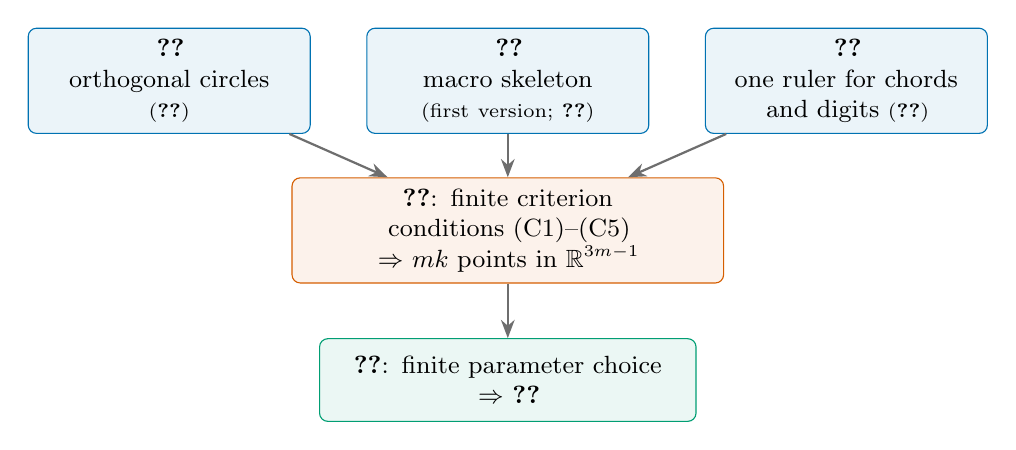
\begin{tikzpicture}[
   box/.style={draw=#1,fill=#1!8,rounded corners=3pt,align=center,
               font=\small,inner sep=4pt,minimum height=1.05cm,text width=3.3cm},
   box/.default=cblue,
   >=Stealth]
 \node[box=cblue] (L1) at (0,0) {\cref{lem:completion}\\ orthogonal circles\\ {\scriptsize(\cref{sec:circle})}};
 \node[box=cblue] (L2) at (4.3,0) {\cref{lem:macro}\\ macro skeleton\\ {\scriptsize(first version; \cref{app:macro})}};
 \node[box=cblue] (L3) at (8.6,0) {\cref{lem:ruler}\\ one ruler for chords\\ and digits {\scriptsize(\cref{sec:ruler})}};
 \node[box=cverm,text width=5.2cm] (C) at (4.3,-1.9) {\cref{thm:criterion}: finite criterion\\ conditions \cond1--\cond5 $\Rightarrow$ $mk$ points in $\R^{3m-1}$};
 \node[box=cgreen,text width=4.5cm] (E) at (4.3,-3.8) {\cref{sec:explicit}: finite parameter choice\\ $\Rightarrow$ \cref{thm:explicit}};
 \draw[->,thick,cgray] (L1) -- (C);
 \draw[->,thick,cgray] (L2) -- (C);
 \draw[->,thick,cgray] (L3) -- (C);
 \draw[->,thick,cgray] (C) -- (E);
\end{tikzpicture}
\caption{Logical structure of the paper.}
\label{fig:roadmap}
\end{figure}

\emph{Notation.} Norms $\norm\cdot$ and inner products $\ip\cdot\cdot$ are
Euclidean; $\opnorm\cdot$ is the operator norm of a matrix. We write
$e_0,\dots,e_{m-1}$ for the standard basis of $\R^m$, indexed from zero.
Given vectors $V_0,\dots,V_{m-1}\in\R^r$, we also write $V$ for the
$r\times m$ matrix with columns $V_A=Ve_A$. For symmetric matrices,
$P\succeq Q$ means that $P-Q$ is positive semidefinite, and $P[x]=x^\T Px$
is the associated quadratic form. $\one_{\mathcal P}$ equals $1$ if the
statement $\mathcal P$ is true and $0$ otherwise. Capital letters $A,B,J$
index clusters ($0\le A<m$) and lower-case $i,j$ index points within a
cluster ($0\le i<k$). Finally, $H_m=\sum_{j=1}^m1/j$ is the $m$-th harmonic
number.

% ===========================================================================
\section{The geometric principle: orthogonal circles}\label{sec:circle}

We want to place one circle of radius $R$ around each macro vertex. Each
circle must tilt into the macro space in a prescribed direction $U_A$,
because the inner products of $U_A$ with the macro edges will produce the
digits. At the same time the circles should lie in mutually orthogonal
planes, so that they do not interact. The following lemma shows that both
requirements can be met with $2m$ extra coordinates, provided the whole
matrix of directions has operator norm at most~$R$.
The Gram-deficit square root is the standard defect-operator completion for
a contraction after rescaling~\cite{Robinson}. The quantitative input here is
the bound on the complete direction matrix~$U$.

\begin{lemma}[Orthogonal-circle completion]\label[lemma]{lem:completion}
Let $R>0$, and let $U$ be a real $r\times m$ matrix with columns
$U_0,\dots,U_{m-1}\in\R^r$ and $\opnorm U\le R$. Put
\[
 W=(R^2I_m-U^\T U)^{1/2},
\]
the positive semidefinite square root. For $0\le A<m$ and $z\in\R$ define
\begin{equation}\label{eq:eta}
 \eta_A(z)=\bigl(U_A\sin z,\;We_A\sin z,\;Re_A\cos z\bigr)
       \in\R^r\oplus\R^m\oplus\R^m.
\end{equation}
Then for all $z,w\in\R$,
\begin{align}
 \norm{\eta_A(z)}&=R,\label{eq:eta-norm}\\
 \ip{\eta_A(z)}{\eta_B(w)}&=0 &&(A\ne B),\label{eq:eta-orthogonal}\\
 \norm{\eta_A(z)-\eta_A(w)}
   &=2R\left|\sin\frac{z-w}{2}\right|.\label{eq:eta-chord}
\end{align}
In words: $\eta_A$ traces a circle of radius $R$ centred at the origin,
and the $m$ circle planes are mutually orthogonal. Only $r+2m$
coordinates are used, however many points are later placed on each
circle.
\end{lemma}

\begin{proof}
The matrix $R^2I_m-U^\T U$ is positive semidefinite because
$\opnorm U\le R$, so $W$ exists, and $U^\T U+W^\T W=R^2I_m$. Put
\[
 a_A=(U_A,\;We_A,\;0),\qquad b_A=(0,\;0,\;Re_A).
\]
Then $\ip{a_A}{a_B}=(U^\T U+W^\T W)_{AB}=R^2\one_{A=B}$ and
$\ip{b_A}{b_B}=R^2\one_{A=B}$, while $\ip{a_A}{b_B}=0$ for all $A,B$.
Thus the $2m$ vectors $a_A,b_A$ are pairwise orthogonal and all have norm
$R$. Since $\eta_A(z)=a_A\sin z+b_A\cos z$, the curve $\eta_A$ is a circle
of radius $R$ in the plane spanned by $a_A$ and $b_A$, and these planes are
mutually orthogonal. The identities
\eqref{eq:eta-norm}--\eqref{eq:eta-chord} follow at once; for the last
one, $\norm{\eta_A(z)-\eta_A(w)}^2=2R^2-2R^2\cos(z-w)=4R^2\sin^2\frac{z-w}2$.
\end{proof}

\begin{figure}[t]
\centering
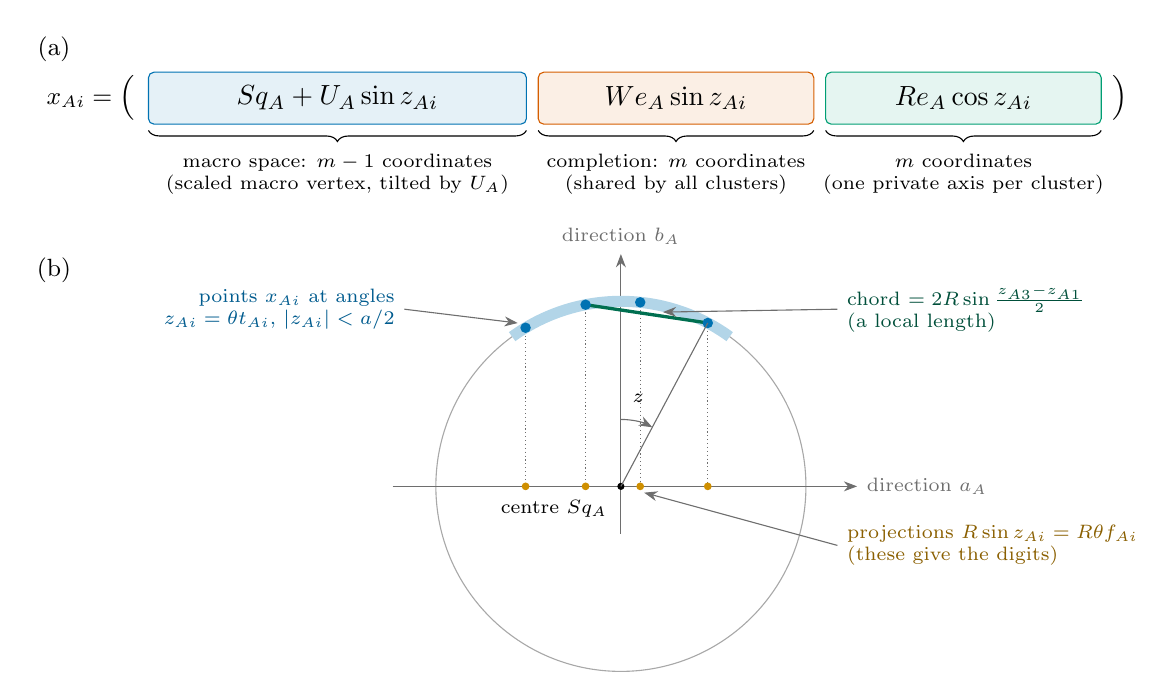
\begin{tikzpicture}[>=Stealth]
 % ---------------- (a) coordinate blocks ----------------
 \begin{scope}
  \node[font=\small] at (-0.6,0.95) {(a)};
  \def\h{0.66}
  \node[font=\small,anchor=east] at (0.55,0.33) {$x_{Ai}=\Bigl($};
  \filldraw[draw=cblue,fill=cblue!10,rounded corners=2pt] (0.6,0) rectangle (5.4,\h);
  \filldraw[draw=cverm,fill=cverm!10,rounded corners=2pt] (5.55,0) rectangle (9.05,\h);
  \filldraw[draw=cgreen,fill=cgreen!10,rounded corners=2pt] (9.2,0) rectangle (12.7,\h);
  \node[font=\small,anchor=west] at (12.72,0.33) {$\Bigr)$};
  \node at (3.0,\h/2) {$Sq_A+U_A\sin z_{Ai}$};
  \node at (7.3,\h/2) {$We_A\sin z_{Ai}$};
  \node at (10.95,\h/2) {$Re_A\cos z_{Ai}$};
  \draw[decorate,decoration={brace,mirror,amplitude=4pt}] (0.6,-0.08) -- (5.4,-0.08)
        node[midway,below=5pt,font=\scriptsize,align=center] {macro space: $m-1$ coordinates\\ (scaled macro vertex, tilted by $U_A$)};
  \draw[decorate,decoration={brace,mirror,amplitude=4pt}] (5.55,-0.08) -- (9.05,-0.08)
        node[midway,below=5pt,font=\scriptsize,align=center] {completion: $m$ coordinates\\ (shared by all clusters)};
  \draw[decorate,decoration={brace,mirror,amplitude=4pt}] (9.2,-0.08) -- (12.7,-0.08)
        node[midway,below=5pt,font=\scriptsize,align=center] {$m$ coordinates\\ (one private axis per cluster)};
 \end{scope}
 % ---------------- (b) one circle ----------------
 \begin{scope}[xshift=6.6cm,yshift=-4.6cm]
  \node[font=\small] at (-7.2,2.75) {(b)};
  \def\Rr{2.35}
  \draw[cgray!60] (0,0) circle (\Rr);
  \draw[cgray,->] (-2.9,0) -- (3.0,0) node[right,font=\scriptsize] {direction $a_A$};
  \draw[cgray,->] (0,-0.6) -- (0,2.95) node[above,font=\scriptsize] {direction $b_A$};
  \fill (0,0) circle (1.3pt);
  \node[font=\scriptsize,anchor=north east] at (-0.05,-0.05) {centre $Sq_A$};
  % the arc used by the cluster (exaggerated)
  \draw[cblue!30,line width=4pt] ({90-36}:\Rr) arc ({90-36}:{90+36}:\Rr);
  \foreach \z/\nm in {-31/0,-11/1,6/2,28/3}{
     \coordinate (P\nm) at ({90-\z}:\Rr);
     \draw[cgray,densely dotted] (P\nm) -- ({\Rr*sin(\z)},0);
     \fill[corange!90!black] ({\Rr*sin(\z)},0) circle (1.4pt);
  }
  \draw[cgreen!70!black,very thick] (P1) -- (P3);
  \foreach \nm in {0,...,3} \fill[cblue] (P\nm) circle (1.9pt);
  \draw[cgray,thin] (0,0) -- (P3);
  \draw[cgray,->] (0,0.85) arc (90:62:0.85);
  \node[font=\scriptsize] at (0.22,1.12) {$z$};
  % labels
  \node[font=\scriptsize,anchor=west,align=left,text=cgreen!50!black] (ch) at (2.75,2.25)
     {chord $=2R\sin\frac{z_{A3}-z_{A1}}2$\\ (a local length)};
  \draw[cgray,thin,->] (ch.west) -- ($(P1)!0.62!(P3)+(0.02,0.05)$);
  \node[font=\scriptsize,anchor=east,align=right,text=cblue!80!black] (pt) at (-2.75,2.25)
     {points $x_{Ai}$ at angles\\ $z_{Ai}=\theta t_{Ai}$, $|z_{Ai}|<a/2$};
  \draw[cgray,thin,->] (pt.east) -- ($(P0)+(-0.1,0.06)$);
  \node[font=\scriptsize,anchor=west,align=left,text=corange!60!black] (pr) at (2.75,-0.75)
     {projections $R\sin z_{Ai}=R\theta f_{Ai}$\\ (these give the digits)};
  \draw[cgray,thin,->] (pr.west) -- ({\Rr*sin(6)+0.05},-0.08);
 \end{scope}
\end{tikzpicture}
\caption{(a) The $3m-1$ coordinates of a point. The first block carries
the scaled macro vertex and the tilt $U_A$; the other two blocks complete
the circles so that they become mutually orthogonal. Indeed, the $2m$
vectors $a_A=(U_A,We_A,0)$ and $b_A=(0,0,Re_A)$ are pairwise orthogonal
and have length $R$, and $x_{Ai}=(Sq_A,0,0)+a_A\sin z_{Ai}+b_A\cos z_{Ai}$.
(b) The circle of cluster $A$, in the plane of $a_A$ and $b_A$ (angles
exaggerated). The points use only a short arc, of angular width at most
$a\le1$. Two quantities are read off
the same angles $z_{Ai}$: chords, which are the local lengths, and
projections onto the tilted direction $a_A$, which produce the digits of
the cross lengths.}
\label{fig:circle}
\end{figure}

\subsection*{Cross distances}
Now choose macro vertices $q_0,\dots,q_{m-1}\in\R^r$ and a scale $S>0$,
and consider points of the form
\begin{equation}\label{eq:points}
 x_{Ai}=(Sq_A,0,0)+\eta_A(z_{Ai}).
\end{equation}
For $A\ne B$, expanding $\norm{x_{Ai}-x_{Bj}}^2$ and using
\eqref{eq:eta-norm}--\eqref{eq:eta-orthogonal} gives the exact identity
\begin{equation}\label{eq:cross-expansion}
 \norm{x_{Ai}-x_{Bj}}^2
 =\underbrace{S^2\norm{q_A-q_B}^2+2R^2}_{\text{depends only on }A,B}
 \;+\;2S\ip{q_A-q_B}{U_A\sin z_{Ai}-U_B\sin z_{Bj}}.
\end{equation}
The first two terms can be prescribed together: if the macro vertices are
chosen with squared distances \emph{shortened} by $2(R/S)^2$, then these
two terms add up to the desired squared macro length. What remains is a
term \emph{linear} in $\sin z_{Ai}$ and $\sin z_{Bj}$, with no interaction
between them. No quadratic or second-harmonic correction is needed.

% ===========================================================================
\section{The macro skeleton}\label{sec:macro}

The macro edges $AB$, $0\le A<B<m$, are labelled in \emph{colexicographic
order}: first by the larger endpoint $B$, then by the smaller endpoint $A$.
Explicitly,
\begin{equation}\label{eq:colex}
 \ell_{AB}=\binom B2+A+1,\qquad D_{AB}=K+\ell_{AB}
 \qquad(0\le A<B<m),
\end{equation}
and we put $D_{BA}=D_{AB}$. The labels $\ell_{AB}$ run through
$1,2,\dots,M$ exactly once, where $M=\binom m2$ (\cref{fig:colex}). The
number $K>0$ is an offset, and $D_{AB}$ is the length that the macro edge
$AB$ will have, in units of $S$.

\begin{figure}[t]
\centering
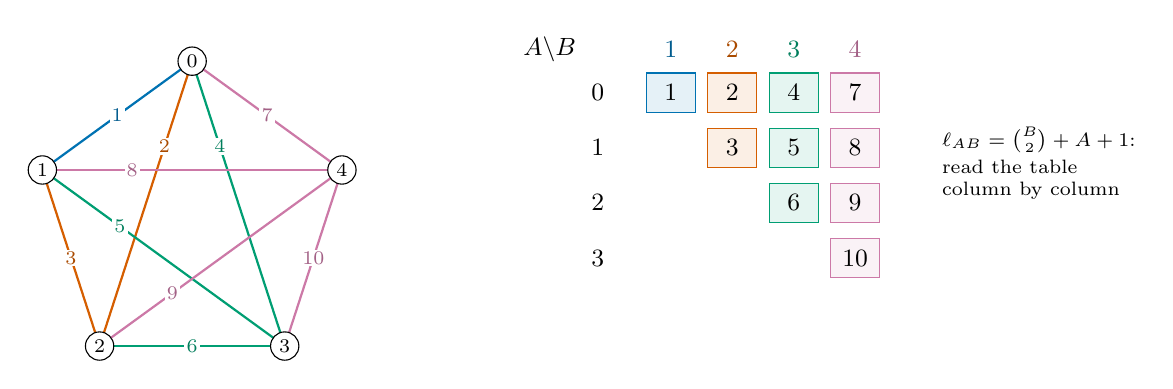
\begin{tikzpicture}[>=Stealth,
   vtx/.style={circle,fill=white,draw=black,inner sep=1.5pt,font=\scriptsize},
   lab/.style={font=\scriptsize,fill=white,inner sep=0.8pt}]
 \begin{scope}
  \foreach \v in {0,...,4} \coordinate (v\v) at ({90+72*\v}:2.0);
  \foreach \a/\b/\l/\c/\p in {0/1/1/cblue/0.5, 0/2/2/cverm/0.3, 1/2/3/cverm/0.5,
          0/3/4/cgreen/0.3, 1/3/5/cgreen/0.32, 2/3/6/cgreen/0.5,
          0/4/7/cpurple/0.5, 1/4/8/cpurple/0.3, 2/4/9/cpurple/0.3, 3/4/10/cpurple/0.5}{
     \draw[\c,thick] (v\a) -- (v\b) node[lab,pos=\p,text=\c!80!black] {\l};
  }
  \foreach \v in {0,...,4} \node[vtx] at (v\v) {$\v$};
 \end{scope}
 \begin{scope}[xshift=5.3cm,yshift=-1.4cm]
  \def\w{0.78}
  \node[font=\small,anchor=east] at (-0.3,3.55) {$A\backslash B$};
  \foreach \b/\c in {1/cblue,2/cverm,3/cgreen,4/cpurple}
     \node[font=\small,text=\c!80!black] at ({\b*\w},3.55) {$\b$};
  \foreach \a in {0,...,3} \node[font=\small] at (-0.15,{3-\a*0.7}) {$\a$};
  \foreach \b/\c in {1/cblue,2/cverm,3/cgreen,4/cpurple}{
     \pgfmathtruncatemacro{\amax}{\b-1}
     \foreach \a in {0,...,\amax}{
        \pgfmathtruncatemacro{\lab}{\b*(\b-1)/2+\a+1}
        \node[draw=\c,fill=\c!10,minimum width=0.62cm,minimum height=0.5cm,font=\small]
             at ({\b*\w},{3-\a*0.7}) {\lab};
     }
  }
  \node[font=\scriptsize,align=left,anchor=west] at (4.1,2.1)
     {$\ell_{AB}=\binom B2+A+1$:\\[2pt] read the table\\ column by column};
 \end{scope}
\end{tikzpicture}
\caption{Colexicographic labels for $m=5$. The edges are listed by
increasing larger endpoint $B$ (one colour for each $B$), and then by
increasing smaller endpoint $A$. The target cross-edge baseline is
$D_{AB}=K+\ell_{AB}$; the realized macro distance is
$\sqrt{D_{AB}^2-2\rho^2}$, where $\rho=R/S$. The target labels are
$K+1,\dots,K+\binom m2$.}
\label{fig:colex}
\end{figure}

The following lemma is the macro input. It says that the colex lengths,
shortened as required by \eqref{eq:cross-expansion}, are realized by an
honest simplex, and it controls two families of vectors attached to it.

\begin{lemma}[Macro skeleton from the first version]\label[lemma]{lem:macro}
Let $m\ge4$, $K>0$ and $\rho\ge0$ satisfy
\begin{equation}\label{eq:macro-gates}
 K\ge m,\qquad K\ge16384H_m^2,
 \qquad \rho\le K/4.
\end{equation}
\begin{enumerate}[label=\textup{(\roman*)},leftmargin=2em]
\item There are affinely independent points $q_0,\ldots,q_{m-1}\in\R^{m-1}$
with
\begin{equation}\label{eq:flattened-metric}
 \norm{q_A-q_B}^2=D_{AB}^2-2\rho^2\qquad(A\ne B).
\end{equation}
\item For each $A$ there are unique vectors $F_A,G_A\in\R^{m-1}$ such that,
for every $J\ne A$,
\begin{equation}\label{eq:anchored-projections}
 \ip{q_A-q_J}{F_A}=D_{AJ}\,\one_{J<A},
 \qquad
 \ip{q_A-q_J}{G_A}=D_{AJ}\,\one_{J>A}.
\end{equation}
\item The $(m-1)\times m$ matrices $F$ and $G$ with these columns satisfy
\begin{equation}\label{eq:FG}
 \opnorm F\le24\sqrt{K+m},\qquad
 \opnorm G\le60\sqrt{K+m}.
\end{equation}
\end{enumerate}
\end{lemma}

This is the first version's macro input~\cite[Lemmas~2--3]{Tripodo}; a complete
proof in the present notation is given in \cref{app:macro}. Part~(ii) is
immediate from~(i): the $m-1$ vectors $q_A-q_J$ $(J\ne A)$ form a basis of
$\R^{m-1}$. The substance is part~(iii). Note that it bounds the
\emph{whole} matrices $F$ and $G$, not just their individual columns. This
is essential, because \cref{lem:completion} needs a bound on the operator
norm of the whole matrix~$U$.

The vector $F_A$ ``sees'' only the macro edges from $A$ down to
smaller vertices, and $G_A$ only those from $A$ up to larger vertices. In a
cross edge between clusters $A<B$, we shall let the smaller endpoint carry
the coarse digit and the larger one the fine digit. Accordingly, given
$s>1$, a cluster size $k$ and an angular scale $\theta>0$, we set
\begin{equation}\label{eq:U}
 U_A=\frac s\theta\bigl(F_A+sk\,G_A\bigr)\qquad(0\le A<m).
\end{equation}
Then for $A<B$ the definitions \eqref{eq:anchored-projections} give the
two projections
\begin{equation}\label{eq:U-projections}
 \ip{q_A-q_B}{U_A}=\frac{s^2k}{\theta}\,D_{AB}
 \quad\text{(coarse)},\qquad
 \ip{q_B-q_A}{U_B}=\frac{s}{\theta}\,D_{AB}
 \quad\text{(fine)}.
\end{equation}
Since $sk\ge1$, the bounds \eqref{eq:FG} give
\begin{equation}\label{eq:U-bound}
 \opnorm U\le\frac s\theta\bigl(24+60sk\bigr)\sqrt{K+m}
 \le\frac{84s^2k\sqrt{K+m}}{\theta}.
\end{equation}

% ===========================================================================
\section{One ruler for local lengths and digits}\label{sec:ruler}

The angles on the circles come from the following ruler. It is a
quadratic-residue construction of Erd\H{o}s--Tur\'an
type~\cite{ErdosTuran}, with a linear term depending on the cluster as in
the first version~\cite{Tripodo}. For an integer $u$ we write $\res u$ for the least
nonnegative residue of $u$ modulo~$p$.

\begin{lemma}[Clustered ruler]\label[lemma]{lem:ruler}
Let $m,k\ge2$ and $L\ge3$ be integers, and let $p$ be a prime with
$2mk<p<4mk$. Define the integers
\begin{equation}\label{eq:ruler}
 y_{Ai}=Lp\,i+\res{i^2+2kAi}
 \qquad(0\le A<m,\ 0\le i<k).
\end{equation}
Then the differences $y_{Aj}-y_{Ai}$, taken over all clusters $A$ and all
$0\le i<j<k$, are positive and pairwise distinct. Moreover, with
\begin{equation}\label{eq:normalized-ruler}
 \kappa=1-\frac1L,\qquad h=\frac{k-\kappa}{2},\qquad
 t_{Ai}=\frac{y_{Ai}}{Lp}-h,
\end{equation}
the normalized positions $t_{Ai}$ satisfy
\begin{equation}\label{eq:digit-raw-bounds}
 |t_{Ai}|\le h<\frac k2,\qquad
 t_{A,i+1}-t_{Ai}>\kappa,\qquad
 t_{A,k-1}-t_{A0}<k-\kappa.
\end{equation}
\end{lemma}

So each row $t_{A0}<\dots<t_{A,k-1}$ is an almost evenly spaced sequence,
with steps between $\kappa=1-1/L$ and $1+1/L$, inside $[-h,h]$; but all
the differences of the underlying integers, across all clusters, are
distinct (\cref{fig:ruler}). Taking $L$ large makes the spacing nearly
uniform.

\begin{proof}
Fix a lag $1\le\delta<k$ and write
$g_{Ai\delta}=y_{A,i+\delta}-y_{Ai}$ for $0\le i<k-\delta$. The residue
parts of $y_{A,i+\delta}$ and $y_{Ai}$ lie in $[0,p)$, and
$(i+\delta)^2+2kA(i+\delta)-i^2-2kAi=\delta(2i+\delta+2kA)$, so
\begin{equation}\label{eq:ruler-window}
 (L\delta-1)p<g_{Ai\delta}<(L\delta+1)p,
 \qquad
 g_{Ai\delta}\equiv\delta\,(2i+\delta+2kA)\pmod p.
\end{equation}
In particular every difference is positive. Differences with different
lags lie in disjoint windows, since $L\ge2$. For a fixed lag, the
integers $2i+\delta+2kA$ lie in $[1,2mk)\subset[1,p)$, and they are
pairwise distinct: $2i+\delta+2kA=2i'+\delta+2kA'$ forces
$i-i'=k(A'-A)$, and as $|i-i'|<k$ this gives $A=A'$ and $i=i'$. Since
$0<\delta<p$, multiplication by $\delta$ is injective modulo $p$, so the
residues of the $g_{Ai\delta}$ are pairwise distinct as well. This proves
that all differences are distinct.

For the bounds, $0\le y_{Ai}\le Lp(k-1)+p-1$, so
$0\le y_{Ai}/(Lp)<k-1+1/L=k-\kappa=2h$; this gives $|t_{Ai}|\le h$. The
consecutive differences satisfy $g_{Ai1}/(Lp)>(L-1)/L=\kappa$ by
\eqref{eq:ruler-window}, and the total range is less than $2h=k-\kappa$.
\end{proof}

\begin{figure}[t]
\centering
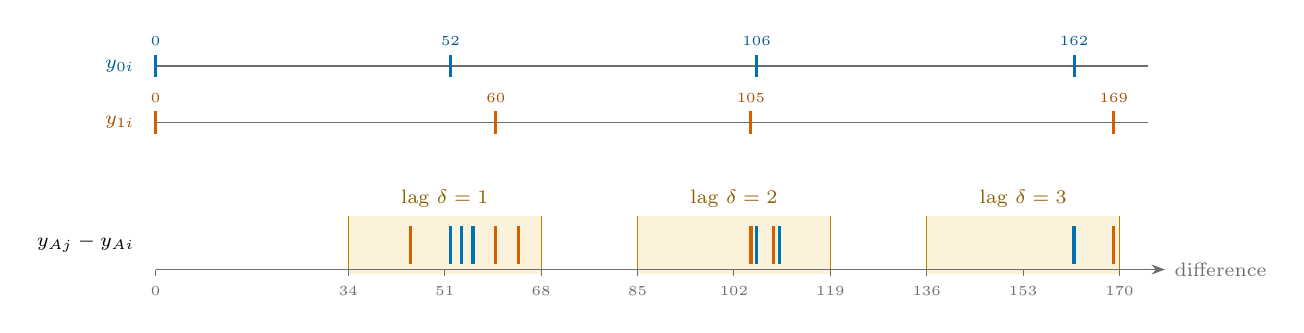
\begin{tikzpicture}[>=Stealth,x=0.072cm,y=1.1cm]
 % ---- the two rulers ----
 \foreach \yy/\col/\A/\marks in {2.35/cblue/0/{0,52,106,162}, 1.7/cverm/1/{0,60,105,169}}{
   \draw[cgray] (0,\yy) -- (175,\yy);
   \foreach \x [count=\ii from 0] in \marks {
     \draw[\col,line width=1.1pt] (\x,\yy-0.13) -- (\x,\yy+0.13);
     \node[font=\tiny,above,text=\col!80!black] at (\x,\yy+0.12) {\x};
   }
   \node[font=\scriptsize,anchor=east,text=\col!80!black] at (-2,\yy) {$y_{\A i}$};
 }
 % ---- the windows and the differences ----
 \foreach \d in {1,2,3}{
   \pgfmathsetmacro{\lo}{(3*\d-1)*17}
   \pgfmathsetmacro{\hi}{(3*\d+1)*17}
   \fill[corange!14] (\lo,-0.05) rectangle (\hi,0.62);
   \draw[corange!80!black,thin] (\lo,-0.05) -- (\lo,0.62) (\hi,-0.05) -- (\hi,0.62);
   \node[font=\scriptsize,text=corange!60!black] at ({(\lo+\hi)/2},0.82) {lag $\delta=\d$};
 }
 \draw[cgray,->] (0,0) -- (178,0) node[right,font=\scriptsize] {difference};
 \foreach \x in {0,34,51,68,85,102,119,136,153,170}
    \draw[cgray] (\x,0) -- (\x,-0.08) node[below,font=\tiny] {\x};
 \foreach \x in {52,54,56,106,110,162} \draw[cblue,line width=1.2pt] (\x,0.06) -- (\x,0.5);
 \foreach \x in {45,60,64,105,109,169} \draw[cverm,line width=1.2pt] (\x,0.06) -- (\x,0.5);
 \node[font=\scriptsize,anchor=east,align=right] at (-2,0.3) {$y_{Aj}-y_{Ai}$};
\end{tikzpicture}
\caption{The ruler of \cref{lem:ruler} for $m=2$ clusters of $k=4$ points,
with $L=3$ and $p=17$. Top: the marks $y_{0i}$ (blue) and $y_{1i}$ (red).
Bottom: all $2\binom42=12$ differences $y_{Aj}-y_{Ai}$. A difference
with lag $\delta=j-i$ lies in the shaded window from $(L\delta-1)p$ to
$(L\delta+1)p$. Inside a window, the quadratic residues keep all
differences apart, even across the two clusters.}
\label{fig:ruler}
\end{figure}

By Bertrand's postulate (for every integer $N\ge2$ there is a prime $p$
with $N<p<2N$), a prime as in \cref{lem:ruler} exists. We now turn the
positions $t_{Ai}$ into angles and digits. Fix $0<a\le1$, which will be
the angular width of every cluster, and put
\begin{equation}\label{eq:sine-digits}
 \theta=\frac ak,\qquad
 z_{Ai}=\theta t_{Ai},\qquad
 f_{Ai}=\frac{\sin z_{Ai}}{\theta}=\frac{\sin(\theta t_{Ai})}{\theta},\qquad
 \gamma=1-\frac{a^2}{8},\qquad \lambda=\kappa\gamma.
\end{equation}
The angle $z_{Ai}$ places the point $x_{Ai}$ on its circle, and $f_{Ai}$ is
its digit. Since $|t_{Ai}|\le h<k/2$, all angles satisfy
$|z_{Ai}|<a/2\le1/2$. On this range the function $t\mapsto\sin(\theta
t)/\theta$ has derivative $\cos(\theta t)\in[\gamma,1]$, because $\cos
u\ge1-u^2/2$. By the mean value theorem, \eqref{eq:digit-raw-bounds}
becomes
\begin{equation}\label{eq:digit-bounds}
 |f_{Ai}|\le h,\qquad
 f_{A,i+1}-f_{Ai}>\lambda,\qquad
 f_{A,k-1}-f_{A0}<k-\kappa.
\end{equation}
So the digits of each cluster increase in steps larger than $\lambda$ (a
number slightly below one) and span an interval shorter than $k$. Since
the angles themselves come from the ruler, there is no separate local
geometry to fit into the construction.

% ===========================================================================
\section{A finite criterion}\label{sec:criterion}

We now assemble the construction. All the numerical requirements are
collected into five inequalities, \cond1--\cond5, on six inputs
$m,L,s,a,C,K$, summarized in \cref{tab:parameters}. The tolerance
$\tau$ is determined by these inputs. Since $k$ occurs in none of the
inequalities, one feasible choice works for every cluster size $k\ge2$.

\begin{table}[t]
\centering
\caption{The parameters of \cref{thm:criterion} and the finite choice
used to prove \cref{thm:explicit} in \cref{sec:explicit}.}
\label{tab:parameters}
\renewcommand{\arraystretch}{1.18}
\small
\begin{tabular}{@{}c>{\raggedright\arraybackslash}p{8.0cm}c@{}}
\toprule
 & role & finite choice\\
\midrule
$m$ & number of clusters; dimension $3m-1$ & $18177\le m\le27265$\\
$k$ & points per cluster & any $k\ge2$\\
$K$ & offset of the macro lengths $D_{AB}=K+\ell_{AB}$ & $\lceil m(m-1)/64\rceil$\\
$s$ & slack factor, $s>1$; scale $S=s^3k^2$ & $9/8$\\
$a$ & angular width of each cluster; $\theta=a/k$ & $49/100$\\
$L$ & spacing factor of the ruler & $12$\\
$C$ & radius constant; radius $R=Cmk^2$ & $101$\\
\midrule
\multicolumn{3}{@{}l}{derived:\quad
 $\kappa=1-1/L,\quad\gamma=1-a^2/8,\quad\lambda=\kappa\gamma,
 \quad M=\binom m2,\quad \rho=R/S=Cm/s^3$}\\
\bottomrule
\end{tabular}
\end{table}

\begin{theorem}[Finite criterion]\label{thm:criterion}
Let $m\ge4$ and $L\ge3$ be integers, and let $s>1$, $0<a\le1$,
$C,K>0$ be real numbers. With $\kappa,\gamma,\lambda,M$ as in
\cref{tab:parameters}, define the slope tolerance
\begin{equation}\label{eq:derived-tau}
 \tau=\sqrt{1-\frac1{s(K+1)}}\ \in(0,1).
\end{equation}
Suppose that
\begin{align}
 \tau s\lambda&>1, \tag{C1}\label{eq:C1}\\
 K&\ge\max\{m,\ 16384H_m^2\}, \tag{C2}\label{eq:C2}\\
 K&\ge4Cm/s^3, \tag{C3}\label{eq:C3}\\
 Cm&\ge\frac{84s^2}{a}\sqrt{K+m}, \tag{C4}\label{eq:C4}\\
 Ca\gamma&>4L. \tag{C5}\label{eq:C5}
\end{align}
Then for every integer $k\ge2$ there is a distance-separated set of $mk$
distinct points in $\R^{3m-1}$ with diameter at most
\begin{equation}\label{eq:finite-diameter}
 \Bigl[s^3(K+M)+\frac{s^2}{2\tau}\Bigr]k^2.
\end{equation}
\end{theorem}

The definition \eqref{eq:derived-tau} makes the cross-length slope
budget an identity. The local-versus-cross guard follows automatically:
by \cond3,
$s^3K\ge4Cm$. Also \cond5, $L\ge3$, $a\le1$ and $\gamma\le1$ give
$Cm\ge Ca>12$. Hence $(4-a)Cm\ge3Cm>36>1$, and therefore
\begin{equation}\label{eq:automatic-guard}
 s^3K\ge4Cm>Cam+1.
\end{equation}

The conditions have the following roles in the proof:
\begin{itemize}[leftmargin=2em,itemsep=1pt]
\item \cond1: a fine step increases the cross length by more than one;
\item \cond2, \cond3: \cref{lem:macro} applies with the shortening
 $\rho=R/S$ required by \eqref{eq:cross-expansion}; \cond3 also
 puts cross lengths above local lengths;
\item \cond4: the radius $R$ is at least $\opnorm U$, so that
 \cref{lem:completion} applies;
\item \cond5: chords of the circles grow by more than one per unit of
 the ruler.
\end{itemize}

\begin{proof}
Fix $k\ge2$. We construct the points and then compare the lengths of all
pairs of edges: local with local, cross with cross, and local with cross.

\smallskip\noindent\emph{Step 1: construction.}
Set
\begin{equation}\label{eq:scales}
 S=s^3k^2,\qquad R=Cmk^2,\qquad
 \rho=\frac RS=\frac{Cm}{s^3},\qquad \theta=\frac ak.
\end{equation}
By \cond2 and \cond3, \cref{lem:macro} applies with this $\rho$. Take its
macro vertices $q_A\in\R^{m-1}$ and the vectors $U_A$ from
\eqref{eq:U}. By \eqref{eq:U-bound} and \cond4,
\[
 \opnorm U\le\frac{84s^2k\sqrt{K+m}}{a/k}
 =\frac{84s^2}{a}\sqrt{K+m}\;k^2\le Cmk^2=R,
\]
so \cref{lem:completion} applies with $r=m-1$. Take the ruler of
\cref{lem:ruler} and the angles $z_{Ai}=\theta t_{Ai}$ of
\eqref{eq:sine-digits}, and define, as in \eqref{eq:points},
\begin{equation}\label{eq:actual-point}
 x_{Ai}=\bigl(Sq_A+U_A\sin z_{Ai},\ \ We_A\sin z_{Ai},\ \ Re_A\cos z_{Ai}\bigr)
 \in\R^{m-1}\oplus\R^m\oplus\R^m,
\end{equation}
where $W=(R^2I_m-U^\T U)^{1/2}$ (\cref{fig:circle}\,(a)). These points lie in
$\R^{3m-1}$.

\smallskip\noindent\emph{Step 2: local edges.}
Let $A$ be a cluster and $i<j$. By \eqref{eq:eta-chord}, the local length
is a chord:
\begin{equation}\label{eq:local-metric}
 \norm{x_{Aj}-x_{Ai}}=2R\sin\frac{z_{Aj}-z_{Ai}}2
 =\phi(y_{Aj}-y_{Ai}),
 \qquad\text{where }\ \phi(g)=2R\sin\frac{\theta g}{2Lp}.
\end{equation}
Thus every local length, in every cluster, is the value of one fixed
function $\phi$ at the corresponding ruler difference $g=y_{Aj}-y_{Ai}$,
which is a positive integer with $g/(Lp)<k$. For $0\le g\le Lpk$ we have
$\theta g/(2Lp)\le a/2$, so
\[
 \phi'(g)=\frac{R\theta}{Lp}\cos\frac{\theta g}{2Lp}
 \ge\frac{R\theta\gamma}{Lp}
 >\frac{Camk\,\gamma}{L\cdot4mk}
 =\frac{Ca\gamma}{4L}>1,
\]
using $R\theta=Camk$, $p<4mk$ and \cond5. By \cref{lem:ruler}, distinct
local edges have distinct integer differences $g$, even when they lie in
different clusters. Hence, by the mean value theorem, any two local
lengths differ by more than one. Likewise every local length is at least
$\phi(1)>\phi(0)+1=1$. Since $2\sin(u/2)\le u$, the local lengths are also
bounded above:
\begin{equation}\label{eq:local-upper}
 \norm{x_{Aj}-x_{Ai}}\le R\,(z_{Aj}-z_{Ai})< R\theta k=Camk^2.
\end{equation}

\smallskip\noindent\emph{Step 3: an exact formula for cross lengths.}
Let $A<B$, and put
\begin{equation}\label{eq:cross-digits}
 \nu=SD_{AB},\qquad T_{AiBj}=s^2k\,f_{Ai}+s\,f_{Bj}.
\end{equation}
In \eqref{eq:cross-expansion}, the shortened metric
\eqref{eq:flattened-metric} with $\rho=R/S$ gives
$S^2\norm{q_A-q_B}^2+2R^2=S^2D_{AB}^2=\nu^2$, and the projections
\eqref{eq:U-projections} give
\[
 2S\ip{q_A-q_B}{U_A\sin z_{Ai}-U_B\sin z_{Bj}}
 =2SD_{AB}\Bigl(\frac{s^2k}\theta\sin z_{Ai}+\frac s\theta\sin z_{Bj}\Bigr)
 =2\nu\,T_{AiBj}.
\]
Therefore
\begin{equation}\label{eq:simple-cross}
 \norm{x_{Ai}-x_{Bj}}=\Phi_\nu(T_{AiBj}),
 \qquad\text{where }\ \Phi_\nu(T)=\sqrt{\nu^2+2\nu T}.
\end{equation}
We now bound the digit sum and the slope of $\Phi_\nu$. Note first that
\cond1 implies $s\kappa\ge s\lambda>1/\tau>1$ and $s>1/\tau$, because
$\lambda\le\kappa\le1$. By \eqref{eq:digit-bounds}, $|T_{AiBj}|\le\Tmax$,
where
\begin{equation}\label{eq:digit-budget}
 \Tmax=s(sk+1)h=\frac{s(sk+1)(k-\kappa)}2,
 \qquad
 2\Tmax=s^2k^2-s(s\kappa-1)k-s\kappa<s^2k^2.
\end{equation}
Every macro length satisfies $D_{AB}\ge K+1$, so $\nu\ge\nu_0=S(K+1)$.
Hence, for $|T|\le\Tmax$ and by \eqref{eq:derived-tau},
\[
 \frac{2|T|}{\nu}<\frac{s^2k^2}{s^3k^2(K+1)}=\frac1{s(K+1)}\le1-\tau^2.
\]
In particular $\nu^2+2\nu T>0$. Since
$\Phi_\nu'(T)=(1+2T/\nu)^{-1/2}$ and $1+2T/\nu\in[\tau^2,2-\tau^2]$, we
obtain
\begin{equation}\label{eq:derivative-bound}
 \tau\le\Phi_\nu'(T)\le\frac1\tau
 \quad\text{and}\quad
 |\Phi_\nu(T)-\nu|\le\frac{\Tmax}\tau
 \qquad(|T|\le\Tmax).
\end{equation}
For the lower bound on the slope we used $2-\tau^2\le\tau^{-2}$, which is
equivalent to $(1-\tau^2)^2\ge0$; the second bound follows from the first
since $\Phi_\nu(0)=\nu$.

\smallskip\noindent\emph{Step 4: cross lengths are separated.}
List the cross edges as in \cref{fig:counter}: first by the label
$\ell_{AB}$ of the macro edge, and within each macro edge by $(i,j)$ in
lexicographic order. We show that each length in this list exceeds the
previous one by more than one. Three kinds of steps occur.

\emph{Fine step:} $(i,j)\to(i,j+1)$. By \eqref{eq:digit-bounds}, $T$
increases by $s(f_{B,j+1}-f_{Bj})>s\lambda$. Since $\nu$ is unchanged,
\eqref{eq:derivative-bound} shows that the length increases by more than
$\tau s\lambda>1$, by \cond1.

\emph{Carry:} $(i,k-1)\to(i+1,0)$. By \eqref{eq:digit-bounds}, $T$
increases by
\[
 s^2k\,(f_{A,i+1}-f_{Ai})-s\,(f_{B,k-1}-f_{B0})
 >s^2k\lambda-s(k-\kappa)
 =s\bigl[(s\lambda-1)k+\kappa\bigr]\ge s\kappa.
\]
So the length increases by more than $\tau s\kappa\ge\tau s\lambda>1$.

\emph{Macro step:} from the last pair of the macro edge with label $\ell$
to the first pair of the macro edge with label $\ell+1$. Here $\nu$
increases by exactly $S$. By \eqref{eq:derivative-bound}, all lengths of
one macro edge lie within $\Tmax/\tau$ of its $\nu$, so the length
increases by at least $S-2\Tmax/\tau$. Using \eqref{eq:digit-budget},
\begin{equation}\label{eq:macro-polynomial}
 S-\frac{2\Tmax}{\tau}
 =s^2\Bigl(s-\frac1\tau\Bigr)k^2
  +\frac{s(s\kappa-1)}{\tau}\,k+\frac{s\kappa}{\tau}
 >1,
\end{equation}
since all three terms are positive and the last one exceeds one.

Consecutive cross lengths in the list therefore differ by more than one,
and so do any two cross lengths.

\smallskip\noindent\emph{Step 5: local versus cross lengths, and the
diameter.} By \eqref{eq:derivative-bound}, \eqref{eq:digit-budget} and
$s>1/\tau$, every cross length is at least
\[
 \nu_0-\frac{\Tmax}{\tau}
 >s^3(K+1)k^2-\frac{s^2k^2}{2\tau}
 =s^3Kk^2+s^2\Bigl(s-\frac1{2\tau}\Bigr)k^2
 >s^3Kk^2\ge(Cam+1)k^2,
\]
the last step by \eqref{eq:automatic-guard}. By \eqref{eq:local-upper}, this exceeds every
local length by more than $k^2>1$. Together with Steps~2 and~4, this
proves that the set is distance-separated; as all lengths are positive,
its $mk$ points are distinct. Finally, the largest macro length is
$D_{AB}=K+M$, and the cross lengths dominate the local ones, so by
\eqref{eq:derivative-bound} and \eqref{eq:digit-budget}
\[
 \diam\{x_{Ai}\}\le S(K+M)+\frac{\Tmax}\tau
 \le\Bigl[s^3(K+M)+\frac{s^2}{2\tau}\Bigr]k^2.
 \qedhere
\]
\end{proof}

\begin{remark}[A derivative bound replaces an additive approximation]\label[remark]{rem:error}
Expanding \eqref{eq:simple-cross} gives
$\Phi_\nu(T)=\nu+T+O(T^2/\nu)$. Here $T$ is of order $k^2$ and so is
$\nu$ (for fixed $m$), so the error term is of order $k^2$ and is
\emph{not} bounded as $k\to\infty$; a linear approximation to the cross
lengths would therefore be useless. The proof never uses one. Within one
macro edge it compares values of the same increasing function
$\Phi_\nu$, and only the slope bounds \eqref{eq:derivative-bound} matter
(\cref{fig:phi}). Between different macro edges, a gap of order $k^2$ is
available. This is what removes the quadratic correction terms of the
original construction.
\end{remark}

\begin{figure}[t]
\centering
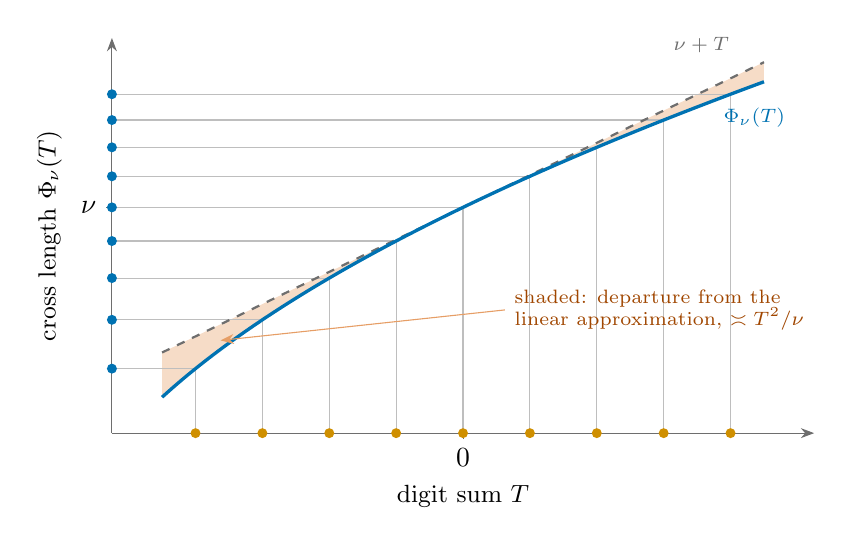
\begin{tikzpicture}
\begin{axis}[
   width=10.5cm,height=6.6cm,
   xmin=-0.42,xmax=0.42,ymin=-0.56,ymax=0.42,
   axis lines=left,
   axis line style={-Stealth,cgray},
   xlabel={digit sum $T$},ylabel={cross length $\Phi_\nu(T)$},
   xlabel style={font=\small},ylabel style={font=\small},
   xtick={0},xticklabels={$0$},
   ytick={0},yticklabels={$\nu$},
   tick style={cgray},
   clip=false]
  % digit grid and its images
  \foreach \t in {-0.32,-0.24,-0.16,-0.08,0,0.08,0.16,0.24,0.32}{
     \pgfmathsetmacro{\v}{sqrt(1+2*\t)-1}
     \edef\temp{\noexpand\draw[cgray!45,thin] (axis cs:\t,-0.56) -- (axis cs:\t,\v) -- (axis cs:-0.42,\v);}
     \temp
  }
  \addplot[name path=lin,domain=-0.36:0.36,samples=2,dashed,cgray,thick] {x};
  \addplot[name path=curve,domain=-0.36:0.36,samples=120,cblue,very thick] {sqrt(1+2*x)-1};
  \addplot[cverm!22] fill between[of=lin and curve];
  \foreach \t in {-0.32,-0.24,-0.16,-0.08,0,0.08,0.16,0.24,0.32}{
     \pgfmathsetmacro{\v}{sqrt(1+2*\t)-1}
     \edef\temp{\noexpand\fill[corange!90!black] (axis cs:\t,-0.56) circle (1.8pt);}
     \temp
     \edef\temp{\noexpand\fill[cblue] (axis cs:-0.42,\v) circle (1.8pt);}
     \temp
  }
  \node[font=\scriptsize,anchor=north west,text=cblue] at (axis cs:0.30,0.27) {$\Phi_\nu(T)$};
  \node[font=\scriptsize,anchor=south east,text=cgray] at (axis cs:0.33,0.36) {$\nu+T$};
  \node[font=\scriptsize,align=left,anchor=north west,text=cverm!75!black] (gap) at (axis cs:0.05,-0.18)
     {shaded: departure from the\\ linear approximation, $\asymp T^2/\nu$};
  \draw[cverm!60,thin,-Stealth] (gap.west) -- (axis cs:-0.29,-0.33);
\end{axis}
\end{tikzpicture}
\caption{The cross length $\Phi_\nu(T)=\sqrt{\nu^2+2\nu T}$ as a function of
the digit sum $T$, with the range of $T/\nu$ greatly exaggerated (in the
construction, $|T|/\nu<1/(2s(K+1))$). The curve departs from the line
$\nu+T$ (shaded) by an amount that grows without bound as $k\to\infty$.
This does not matter: the proof only uses that $\Phi_\nu$ is increasing
with slope in $[\tau,1/\tau]$. Equally spaced digit sums (orange) are
therefore sent to lengths (blue) whose spacings change by a factor of at
most $1/\tau$, so separated digit sums give separated lengths.}
\label{fig:phi}
\end{figure}

% ===========================================================================
\section{A concrete choice of parameters}\label{sec:explicit}

We verify \cref{thm:criterion} for every $m\ge18177$ with
\begin{equation}\label{eq:explicit-parameters}
 s=\frac98,\quad a=\frac{49}{100},\quad L=12,\quad
 C=101,\quad
 K=\Bigl\lceil\frac{m(m-1)}{64}\Bigr\rceil.
\end{equation}
These simple rational values reduce the radius budget while retaining
strict margins in every condition. They give $\kappa=11/12$,
$\gamma=77599/80000$ and $\lambda=853589/960000$.

\emph{Preliminary bounds.} Grouping the terms of $H_{18177}$ into the
dyadic blocks $[2^t,2^{t+1})$, each of which contributes at most one,
gives $H_{18177}\le16<18177/1100$. Since $H_{m+1}=H_m+1/(m+1)$ and
$1/(m+1)\le1/1100$,
induction on $m$ gives
\[
 H_m\le\frac m{1100}\qquad(m\ge18177).
\]
From $m(m-1)/64\le K<m(m-1)/64+1$ we also get
\begin{equation}\label{eq:explicit-K}
 K\ge284m,\qquad K+m\le\frac{m^2}{63},\qquad
 K\ge\frac{m(m-1)}{64}\ge16384\Bigl(\frac m{1100}\Bigr)^2.
\end{equation}
The first holds since $m-1\ge18176=64\cdot284$. The second reduces to
$m^2\ge3969m+4032$, and the third to
$(m-1)/m\ge64\cdot16384/1100^2$; both follow at $m=18177$ and remain
true as $m$ increases.

For a convenient rational lower bound on the derived tolerance, put
$\tau_*=9999/10000$. By $K\ge284m$ and $m\ge18177$,
\[
 \frac1{s(K+1)}\le\frac8{46460421}
 <\frac{19999}{100000000}=1-\tau_*^2,
 \qquad\text{so }\tau>\tau_*.
\]

\emph{The five conditions.}
\begin{itemize}[leftmargin=2em,itemsep=2pt]
\item[\cond1] $\tau s\lambda>\tau_*s\lambda
 =1+\frac{5109233}{25600000000}>1$.
\item[\cond2] $K\ge284m\ge m$, and
 $K\ge16384(m/1100)^2\ge16384H_m^2$ by \eqref{eq:explicit-K}.
\item[\cond3] $4C/s^3=206848/729=284-188/729<284$, so
 $K\ge284m>4Cm/s^3$.
\item[\cond4] By \eqref{eq:explicit-K},
 $\frac{84s^2}{a}\sqrt{K+m}\le\frac{84s^2}{a\sqrt{63}}\,m<28m<101m=Cm$.
\item[\cond5] $\frac{Ca\gamma}{4L}
 =1+\frac{37451}{384000000}>1$.
\end{itemize}

\emph{The diameter.} Put $c_*=s^3(33/64)=24057/32768$. Since
$K<M/32+1$ and $M=m(m-1)/2$, the bound \eqref{eq:finite-diameter}
gives, for all $m\ge18177$ and $k\ge2$, a distance-separated set $X$
of $mk$ points in $\R^{3m-1}$ with
\begin{equation}\label{eq:explicit-diameter}
 \diam X
 <\bigl[c_*m(m-1)+s^3+s^2/(2\tau_*)\bigr]k^2
 <c_*(mk)^2.
\end{equation}
The last comparison holds already for $m\ge4$, since
$4c_*-(s^3+s^2/(2\tau_*))=8008623/9101312>0$. This keeps the leading coefficient
visible instead of replacing it by the looser $147/200$ finite-set cap.

\begin{proof}[Proof of \cref{thm:explicit}]
Given $n\ge36354$, put
\[
 k=\Bigl\lfloor\frac n{18177}\Bigr\rfloor,\qquad
 m=\Bigl\lceil\frac nk\Bigr\rceil.
\]
Writing $n=18177k+b$ with $0\le b<18177$, we have $k\ge2$ and
$m=18177+\lceil b/k\rceil$, and hence
\[
 18177\le m\le18177+\lceil18176/2\rceil=27265,\qquad
 n\le mk<n+k\le\Bigl(1+\frac1{18177}\Bigr)n.
\]
Take the $mk$-point set given by \eqref{eq:explicit-diameter}, keep any
$n$ of its points, and pad with zero coordinates up to dimension
$3\cdot27265-1=81794$. Passing to a subset preserves
\eqref{eq:separated} and cannot increase the diameter. Therefore
\[
 \diam X<c_*\Bigl(\frac{18178}{18177}\Bigr)^2n^2
 =\frac{220816318833}{300740452352}n^2
 <\frac{147}{200}\,n^2.
 \qedhere
\]
\end{proof}

% ===========================================================================
\section{What the method does not give}\label{sec:scope}

The completion lemma holds in every Euclidean space, but using it has a
dimension cost: it consumes $m$ mutually orthogonal circle planes, in
addition to at most $m-1$ macro directions. The explicit theorem uses
$m\le27265$, so this mechanism does not produce a counterexample in a
prescribed low dimension.

In fact, within this construction the dependence on $m$ cannot be removed
by a change of coordinates. If each cluster has at least three points,
the differences of points in cluster $A$ span the plane of its circle
(three distinct points of a circle are never collinear). These $m$ planes
are mutually orthogonal, so the affine span of the whole configuration
has dimension at least $2m$. This is a limitation of the present
mechanism, not an impossibility theorem for other constructions.

There is, however, a genuine obstruction in one dimension: there, the
coefficient $1$ conjectured by Erd\H{o}s is correct. The following short
proof does not require the points to be integers.

\begin{proposition}[The line]\label[proposition]{prop:line}
Every distance-separated set $X\subset\R$ with $|X|=n\ge4$ satisfies
\[
 \diam X\ge n^2-3n^{3/2}.
\]
In particular $\liminf_{n\to\infty}\Delta_1(n)/n^2\ge1$.
\end{proposition}

\begin{proof}
Write $X=\{x_1<\cdots<x_n\}$, let $D=x_n-x_1$, and put
$w=\lfloor\sqrt n\rfloor$. Consider the \emph{short} lengths
$x_{i+j}-x_i$ with $1\le j\le w$ and $1\le i\le n-j$. There are
\[
 Q=\sum_{j=1}^w(n-j)=wn-\frac{w(w+1)}2
\]
of them. They are pairwise separated by at least one and are all at least
one (as in \eqref{eq:counting}), so their sum is at least
$1+2+\dots+Q=Q(Q+1)/2$.

On the other hand, each length $x_{i+j}-x_i$ is a sum of $j$ consecutive
gaps $x_{t+1}-x_t$, and for fixed $j$ each gap occurs in at most $j$ of
these sums. So the lengths with a fixed $j$ add up to at most $jD$, and
all short lengths add up to at most $(1+\dots+w)D=w(w+1)D/2$. Comparing
the two bounds,
\[
 D\ge\frac{Q(Q+1)}{w(w+1)}
 \ge\frac{w}{w+1}\Bigl(n-\frac{w+1}2\Bigr)^2
 \ge n^2-\frac{n^2}{w+1}-n(w+1).
\]
Finally $\sqrt n<w+1\le\sqrt n+1$, so
$D\ge n^2-n^{3/2}-n^{3/2}-n\ge n^2-3n^{3/2}$.
\end{proof}

For $d\ge2$ the present argument leaves open the exact asymptotic
behaviour of $\Delta_d(n)/n^2$, the least dimension in which the
conjectured lower bound fails, and in particular the planar case.

\section*{Acknowledgments}

The author thanks Boon Suan Ho for helpful comments on an earlier draft of this manuscript.

\section*{Attribution and verification scope}

The colex metric, its quantitative Gram reserves, and the fine and coarse
incidence families $F_A,G_A$ come from the first version of this
paper~\cite{Tripodo}. Its clustered quadratic-residue ruler is retained
with a free principal spacing parameter. The orthogonal-circle organization, the use of a
single ruler for both local lengths and digits, and the derivative-based
comparison of cross lengths are the modifications developed in this paper. The positive-semidefinite
completion itself is elementary linear algebra.

This manuscript was developed with substantial AI assistance in mathematical
exploration, proof engineering, source comparison, and writing. An AI-generated
simplification of the construction and readability rewrite informed the revised
construction and presentation, with permission to use it. The finite theorem
stated here was checked in Lean~4 at the finite-proof source pin below. These checks do not
constitute independent human proof or priority review. The concrete finite
conclusion of \cref{thm:explicit} has a
Lean~4 proof in the \href{https://github.com/jjtripodo-lgtm/erdos-670-fixed-dimension/tree/f1604c368efce996a9af4d46f581e676e49054f5/lean}{accompanying source bundle}
(public source commit \texttt{f1604c3}), under the exact declaration
\href{https://github.com/jjtripodo-lgtm/erdos-670-fixed-dimension/blob/f1604c368efce996a9af4d46f581e676e49054f5/lean/Erdos488/Geometry/SeparatedDistances/FixedDimension/Pass5FixedDimension670.lean}{\texttt{pass5\_fixed\_dimension\_erdos\_670}}.
It certifies an injective configuration, minimum distinct-point distance
at least one, separation of genuinely distinct unordered edges, and the
actual set diameter bound. Sixteen new source modules passed a fresh
trust-zero replay, and a scoped build passed with cached upstream imports.
Neither the Lean check nor this manuscript is an independent specialist
proof or priority review. The supplementary rational and small-model
checks alone are not proof certificates.

% ===========================================================================
\appendix
\section{Proof of the macro input}\label{app:macro}

We prove \cref{lem:macro}, following the first version's macro
estimates~\cite[Lemmas~2--3]{Tripodo}. None of the cluster geometry of
the main text is used here. The plan is as follows.
\begin{enumerate}[leftmargin=2em,itemsep=1pt]
\item Compute the Gram matrix $\Gamma$ of the \emph{increments}
 $q_j-q_{j-1}$ that the colex distances would require
 (\cref{sec:app-gram}).
\item Show that $\Gamma$ is dominated by its tridiagonal part, and that
 this part contains two ``reserves'' of positivity: one large
 enough to pay for the shortening by $2\rho^2$, and one diagonal reserve
 (\cref{sec:app-reserves}). This proves part~(i).
\item Use the diagonal reserve to bound the vectors $F_A,G_A$ all at once,
 through their projections on the increments (\cref{sec:app-projections}).
 This proves part~(iii).
\end{enumerate}
Throughout, $m\ge4$ and $K,\rho$ satisfy \eqref{eq:macro-gates}. Since
$H_m\ge1$, the harmonic gate implies $K\ge16384>10$, as used below. Vectors
$x\in\R^{m-1}$ are indexed $x_1,\dots,x_{m-1}$, and $e_A$ $(0\le A<m)$
denotes the standard basis of $\R^m$.

\subsection{The increment Gram matrix}\label{sec:app-gram}

Let $\partial$ be the $(m-1)\times m$ matrix whose $j$-th row is
$e_{j-1}^\T-e_j^\T$ $(1\le j<m)$. For a symmetric $m\times m$ matrix
$\mathbf D$ with zero diagonal, the matrix $-\frac12\partial\mathbf
D\partial^\T$ is the Gram matrix that the increments must have: if points
$q_A$ satisfy $\norm{q_A-q_B}^2=\mathbf D_{AB}$, then
$\ip{q_i-q_{i-1}}{q_j-q_{j-1}}=(-\frac12\partial\mathbf D\partial^\T)_{ij}$,
by the polarization identity. This is Schoenberg's Euclidean-distance
criterion in consecutive-increment coordinates~\cite[Theorem~1]{Schoenberg}.

Let $\mathbf D$ have entries $D_{AB}^2$ off the diagonal, put
$\Gamma=-\frac12\partial\mathbf D\partial^\T$, and write
\[
 D_j=D_{j-1,j}=K+\frac{j(j+1)}2\qquad(1\le j<m)
\]
for the lengths of the consecutive macro edges. Since
$D_{j-1,j+1}=D_j+j$ and $D_{j,j+1}=D_j+j+1$, a direct computation gives
\begin{equation}\label{eq:gram-entries}
 \Gamma_{jj}=D_j^2,\qquad
 \Gamma_{j,j+1}=-c_j,\quad\text{where }\ c_j=\tfrac12(D_j+1)^2+j.
\end{equation}
If $i\le j-2$, the four lengths $D_{i-1,j-1},D_{i-1,j},D_{i,j-1},D_{ij}$ have
the form $\alpha,\beta,\alpha+1,\beta+1$ with $\beta-\alpha=j-1$, and
therefore $\Gamma_{ij}=-(j-1)$. In other words, $\Gamma_{ij}=-(\max\{i,j\}-1)$
whenever $|i-j|\ge2$.

\subsection{Two reserves of positivity}\label{sec:app-reserves}

Split $\Gamma=\mathsf B-\mathsf N$, where the \emph{band} $\mathsf B$
keeps the diagonal and the two neighbouring diagonals of $\Gamma$, and the
\emph{far part} $\mathsf N$ has entries $\max\{i,j\}-1$ for $|i-j|\ge2$
and zero otherwise. Completing squares in $-2c_jx_jx_{j+1}$ gives
\begin{equation}\label{eq:tridiagonal}
 \mathsf B[x]=\sum_{j=1}^{m-2}c_j(x_j-x_{j+1})^2
              +\sum_{j=1}^{m-1}\alpha_jx_j^2+c_{m-1}x_{m-1}^2,
\end{equation}
where $c_{m-1}$ is given by the same formula as the other $c_j$,
$\alpha_j=D_j^2-c_j-c_{j-1}$ with $c_0=0$, and explicitly
\[
 \alpha_1=\frac{K^2}2-2,\qquad \alpha_2=-4,\qquad
 \alpha_j=(j-2)K+\frac{j^3}2-j^2-2j\quad(j\ge3).
\]

\emph{The band dominates a diagonal form.} Define
$\Omega=\diag(\omega_1,\dots,\omega_{m-1})$ by
\[
 \omega_1=\omega_2=\frac{K^2}{24},\qquad \omega_j=\frac{Kj+j^3}{24}\quad(j\ge3).
\]
We claim $\mathsf B\succeq\Omega$. The terms of \eqref{eq:tridiagonal}
involving only $x_1,x_2$ are $c_1(u-v)^2+\alpha_1u^2-4v^2$, with
$u=x_1$, $v=x_2$. Since $c_1,\alpha_1\ge K^2/4$ and
$(u-v)^2+u^2\ge(u^2+v^2)/3$,
\[
 c_1(u-v)^2+\alpha_1u^2-4v^2
 \ge\frac{K^2}{12}(u^2+v^2)-4v^2
 \ge\frac{K^2}{24}(u^2+v^2)
\]
for $K\ge10$. For $j\ge3$ we have $\alpha_j\ge\omega_j$, because
\[
 24(\alpha_j-\omega_j)=(23j-48)K+11j^3-24j^2-48j,
\]
which is positive at $j=3$ (it equals $21K-63$), and has both terms
nonnegative for $j\ge4$. All remaining terms of \eqref{eq:tridiagonal}
are nonnegative.

\emph{The far part is small.} Put $\sigma_0=\sum_j\omega_j^{-1}$ and
$\sigma_2=\sum_jj^2\omega_j^{-1}$. For $K\ge10$,
\[
 \sigma_0\le\frac{48}{K^2}+\frac{24H_m}{K}\le\frac{29H_m}{K},
 \qquad
 \sigma_2\le\frac{120}{K^2}+24H_m\le26H_m.
\]
With $b_0=\sum_j|x_j|$ and $b_1=\sum_jj|x_j|$ we have
$|\mathsf N[x]|\le\sum_{i,j}\max\{i,j\}|x_i||x_j|\le2b_0b_1$, while
weighted Cauchy--Schwarz gives $b_0^2\le\sigma_0\Omega[x]$ and
$b_1^2\le\sigma_2\Omega[x]$. Therefore
\begin{equation}\label{eq:remainder}
 |\mathsf N[x]|
 \le2\sqrt{\sigma_0\sigma_2}\,\Omega[x]
 \le\frac{\sqrt{754}}{64}\,\Omega[x]
 \le\tfrac12\Omega[x]\le\tfrac12\mathsf B[x],
\end{equation}
using $K\ge16384H_m^2$ (so that $\sqrt{29\cdot26}\,H_m/\sqrt K\le\sqrt{754}/128$)
and $754<1024$. Hence
\[
 \Gamma\succeq\tfrac12\mathsf B.
\]

\emph{First reserve: a path energy.} Let $\Pi$ be the quadratic form
\[
 \Pi[x]=D_1^2x_1^2+\sum_{j=1}^{m-2}D_j^2(x_j-x_{j+1})^2+D_{m-1}^2x_{m-1}^2.
\]
In \eqref{eq:tridiagonal}, bound $-4x_2^2\ge-8x_1^2-8(x_2-x_1)^2$. Since
$\alpha_1-8\ge D_1^2/4$, $c_1-8\ge D_1^2/4$, $c_j\ge D_j^2/4$ for all $j$,
and $\alpha_j\ge0$ for $j\ge3$, this proves
\begin{equation}\label{eq:path-reserve}
 \mathsf B\succeq\tfrac14\Pi.
\end{equation}

\emph{Second reserve: a diagonal.} For every $j$,
\begin{equation}\label{eq:diagonal-reserve}
 D_j^2\le36(K+m)\,\omega_j,
 \qquad\text{hence}\qquad
 \mathsf B\succeq\Omega\succeq\frac{\diag(D_1^2,\ldots,D_{m-1}^2)}{36(K+m)}.
\end{equation}
For $j=1,2$ the first inequality is immediate. For $j\ge3$, use
$D_j\le K+j^2\le(K+m)j$ to get the stronger bound
$D_j^2\le(K+j^2)(K+m)j=(K+m)(Kj+j^3)$.

\emph{Paying for the shortening.} Shortening every squared distance by
$2\rho^2$ replaces $\mathbf D$ by $\mathbf D_\rho$, with entries
$D_{AB}^2-2\rho^2$ off the diagonal. Since the rows of $\partial$ sum to
zero, the new increment Gram matrix is
\[
 \Gamma_\rho=-\tfrac12\partial\mathbf D_\rho\partial^\T
 =\Gamma-\rho^2\partial\partial^\T.
\]
Now $\partial\partial^\T[x]=x_1^2+\sum_j(x_j-x_{j+1})^2+x_{m-1}^2\le
\Pi[x]/K^2$, because every $D_j\ge K$. As $\rho\le K/4$, the subtraction
costs at most $\Pi/16\preceq\mathsf B/4$, by \eqref{eq:path-reserve}.
Combining this with $\Gamma\succeq\mathsf B/2$ and the two reserves,
\begin{equation}\label{eq:both-reserves}
 \Gamma_\rho\succeq\tfrac14\mathsf B\succeq\tfrac1{16}\Pi\succ0,
 \qquad
 \Gamma_\rho\succeq
     \frac{\diag(D_1^2,\ldots,D_{m-1}^2)}{144(K+m)}.
\end{equation}
Here $\Pi\succ0$ because $\Pi\succeq K^2\partial\partial^\T$ and $\partial$
has full row rank.

\emph{Proof of part (i).} Since $\Gamma_\rho\succ0$, we may write
$\Gamma_\rho=\mathsf V^\T\mathsf V$ for an invertible
$(m-1)\times(m-1)$ matrix $\mathsf V$ with columns $v_1,\dots,v_{m-1}$
(for instance, by Cholesky factorization). Put $q_0=0$ and
$q_A=v_1+\dots+v_A$. For $A<B$ let $u_{AB}=\sum_{j=A+1}^Be_j\in\R^{m-1}$;
then $\partial^\T u_{AB}=e_A-e_B$, and so
\[
 \norm{q_B-q_A}^2
 =\Gamma_\rho[u_{AB}]
 =-\tfrac12(e_A-e_B)^\T\mathbf D_\rho(e_A-e_B)
 =D_{AB}^2-2\rho^2.
\]
The increments $v_j=q_j-q_{j-1}$ are linearly independent, so the points
$q_A$ are affinely independent.

\subsection{Bounding all projections at once}\label{sec:app-projections}

Let $Y_0,\dots,Y_{m-1}\in\R^{m-1}$ be vectors, and record their
projections on the increments in the $(m-1)\times m$ matrix
\[
 Z_{jA}=\ip{q_j-q_{j-1}}{Y_A},\qquad\text{that is,}\qquad Z=\mathsf V^\T Y.
\]
As $\mathsf V$ is invertible, $Z$ determines $Y$, and
$Y^\T Y=Z^\T(\mathsf V^\T\mathsf V)^{-1}Z=Z^\T\Gamma_\rho^{-1}Z$. Writing
$\mathsf P=\diag(D_1,\dots,D_{m-1})$, the second inequality in
\eqref{eq:both-reserves} gives
$\Gamma_\rho^{-1}\preceq144(K+m)\mathsf P^{-2}$, and hence
\begin{equation}\label{eq:whole-solve}
 \opnorm Y\le12\sqrt{K+m}\,\opnorm{\mathsf P^{-1}Z}.
\end{equation}
So it suffices to show that the projection matrices of $F$ and $G$,
normalized by $\mathsf P^{-1}$, have bounded operator norm.

Taking consecutive differences of the defining equations
\eqref{eq:anchored-projections} (with the convention that the right-hand
sides vanish for $J=A$) gives, for $1\le j<m$ and $0\le A<m$,
\begin{align*}
 Z^F_{jA}&=D_j\,\one_{A=j}-\one_{A>j},\\
 Z^G_{jA}&=-D_j\,\one_{A=j-1}-(j-1)\,\one_{A<j-1}.
\end{align*}
For example, for $A>j$ we get $Z^F_{jA}=D_{j-1,A}-D_{jA}=-1$, because the
colex labels of $\{j-1,A\}$ and $\{j,A\}$ differ by one. The columns $F_0$
and $G_{m-1}$ vanish. Delete them, and index the remaining columns by
$1,\dots,m-1$ (column $A$ of $Z^F$, and column $A-1$ of $Z^G$, become
column $A$). The two projection matrices become
\[
 Z_{\mathrm{fine}}=\mathsf P-\mathsf E_+,\qquad
 Z_{\mathrm{coarse}}=-(\mathsf P+\mathsf E_-),
\]
where $(\mathsf E_+)_{ij}=\one_{i<j}$ and
$(\mathsf E_-)_{ij}=(i-1)\one_{j<i}$.

For the first matrix, the Frobenius norm gives
$\opnorm{\mathsf P^{-1}\mathsf E_+}\le m/K\le1$, as all entries of
$\mathsf P^{-1}\mathsf E_+$ are at most $1/K$. For the second,
\[
 0\le(\mathsf P^{-1}\mathsf E_-)_{ij}
 =\frac{i-1}{D_i}\one_{j<i}
 \le\frac2i\one_{j<i}
\]
since $D_i\ge i(i+1)/2$. The finite Hardy matrix
$\mathcal H_{ij}=i^{-1}\one_{j<i}$ has operator norm at most $2$ by the
weighted Schur test~\cite{Schur,Sinnamon}. For completeness, take
the weights $w_j=j^{-1/2}$; by comparison with integrals,
\[
 \sum_{j<i}\frac{w_j}{i}\le2w_i,
 \qquad \sum_{i>j}\frac{w_i}{i}\le2w_j.
\]
For any real vector $x$, Cauchy--Schwarz with these weights then gives
\[
 \sum_i\Bigl(\sum_j \mathcal H_{ij}x_j\Bigr)^2
 \le\sum_i\Bigl(\sum_j\mathcal H_{ij}w_j\Bigr)
          \Bigl(\sum_j\mathcal H_{ij}\frac{x_j^2}{w_j}\Bigr)
 \le\sum_j\frac{x_j^2}{w_j}\sum_i2w_i\mathcal H_{ij}
 \le4\sum_jx_j^2.
\]
A matrix with nonnegative entries bounded by those of $2\mathcal H$ has
operator norm at most $2\opnorm{\mathcal H}$ (apply it to $|x|$), so
$\opnorm{\mathsf P^{-1}\mathsf E_-}\le4$.

Thus $\opnorm{\mathsf P^{-1}Z_{\mathrm{fine}}}\le2$ and
$\opnorm{\mathsf P^{-1}Z_{\mathrm{coarse}}}\le5$, and
\eqref{eq:whole-solve} gives $\opnorm F\le24\sqrt{K+m}$ and
$\opnorm G\le60\sqrt{K+m}$; restoring the zero columns does not change
the norms. This proves \eqref{eq:FG} and completes the proof of
\cref{lem:macro}.
\qed

\begin{thebibliography}{9}
\enlargethispage{3\baselineskip}

\bibitem{Erdos}
P.~Erd\H{o}s,
\emph{Some unsolved problems},
in \emph{Combinatorics, Geometry and Probability: A Tribute to Paul Erd\H{o}s},
B.~Bollob\'as and A.~Thomason (eds.),
Cambridge University Press, 1997, pp.~1--10, Problem~20.
\href{https://doi.org/10.1017/CBO9780511662034.004}{doi:10.1017/CBO9780511662034.004}.

\bibitem{ErdosTuran}
P.~Erd\H{o}s and P.~Tur\'an,
\emph{On a problem of Sidon in additive number theory, and on some related problems},
J. London Math. Soc. \textbf{16} (1941), 212--215.
\href{https://doi.org/10.1112/jlms/s1-16.4.212}{doi:10.1112/jlms/s1-16.4.212}.

\bibitem{Ho}
Boon Suan Ho,
\emph{Erd\H{o}s's diameter conjecture for separated distances fails in high dimensions},
2026, \href{https://arxiv.org/abs/2604.15305v1}{arXiv:2604.15305v1}.

\bibitem{Tripodo}
J.~Tripodo,
\emph{Separated Euclidean distances with diameter below $0.74n^2$ in a fixed dimension},
research manuscript, 12 October 2026.
Public source snapshot \TripodoCommit,
\href{https://github.com/jjtripodo-lgtm/erdos-670-fixed-dimension/tree/1e73a12ff1076dd11affadbf619ddbbef587133e}{\texttt{jjtripodo-lgtm/erdos-670-fixed-dimension}},
\texttt{paper/fixed\_dimension\_670.tex}.

\bibitem{Schoenberg}
I.~J. Schoenberg,
\emph{Remarks to Maurice Fr\'echet's article ``Sur la d\'efinition axiomatique d'une classe d'espace distanci\'es vectoriellement applicable sur l'espace de Hilbert''},
Ann. of Math. (2) \textbf{36} (1935), 724--732.
\href{https://doi.org/10.2307/1968654}{doi:10.2307/1968654}.

\bibitem{Schur}
I.~Schur,
\emph{Bemerkungen zur Theorie der beschr\"ankten Bilinearformen mit unendlich vielen Ver\"anderlichen},
J. Reine Angew. Math. \textbf{140} (1911), 1--28.
\href{https://doi.org/10.1515/crll.1911.140.1}{doi:10.1515/crll.1911.140.1}.

\bibitem{Sinnamon}
G.~Sinnamon,
\emph{Schur's lemma and best constants in weighted norm inequalities},
Le Matematiche \textbf{57} (2002), fasc.~II, 185--204.
\url{https://lematematiche.dmi.unict.it/index.php/lematematiche/article/view/207}.

\bibitem{Robinson}
P.~L. Robinson,
\emph{Julia operators and Halmos dilations}, arXiv:1803.09329v1, 2018.
\url{https://arxiv.org/abs/1803.09329v1}.

\bibitem{ErdosLenz}
P.~Erd\H{o}s,
\emph{On sets of distances of $n$ points in Euclidean space},
Publ. Math. Inst. Hungar. Acad. Sci. \textbf{5} (1960), 165--169.
\url{https://users.renyi.hu/~p_erdos/1960-08.pdf}.

\end{thebibliography}
\end{document}
